\ifx\twocol\undefined
\documentclass[12pt,letterpaper]{article}
\newcommand{\twocol}{0}
\else
\documentclass[8pt,twocolumn,letterpaper]{article}  % TWO COLUMN VERSION
\renewcommand{\twocol}{true}
\fi

\usepackage{amsmath}
\usepackage[pdftex]{color,graphicx}
\usepackage{verbatim}
\usepackage{setspace}
\usepackage{subfig}
\usepackage{algorithm}
\usepackage{algorithmicx}
\usepackage{algpseudocode}
\usepackage{ifthen}

% Include other packages here, before hyperref.

% If you comment hyperref and then uncomment it, you should delete
% egpaper.aux before re-running latex.  (Or just hit 'q' on the first latex
% run, let it finish, and you should be clear).
% \usepackage[pagebackref=true,breaklinks=true,letterpaper=true,colorlinks,bookmarks=false]{hyperref}
% \usepackage[colorlinks]{hyperref}

%%%THESIS%%% represent comment for thesis writing.
%\textcolor{red}{...}   represent comment for further elaborate.

% Define user command: This is for Bibliograph
\newcommand{\bbauth}[1]{\textrm{#1}}
\newcommand{\bbtitl}[1]{\textrm{#1}}
\newcommand{\bbjour}[1]{\textit{#1}}

%%%%%%%%%%%%%%%%%%%%%%%%%%%%%%%%
%%%%%%   GLOBAL SETTING  %%%%%%%
%%%%%%%%%%%%%%%%%%%%%%%%%%%%%%%%
%\onehalfspace
\doublespace

\begin{document}
%%%%%%%%%%%%%%%%%%%%%%%%%%%%%%%%
%%%%%%   Title         %%%%%%%%%
%%%%%%%%%%%%%%%%%%%%%%%%%%%%%%%%
\title{\textbf{Light-Weight 3D Building Reconstruction From Range Data}}
\author{
\\
\textbf{Weihong Li}
\\
\\
Department of Computer Science 
\\
The Graduate Center
\\
The City University of New York
\\
365 Fifth Avenue
\\
New York, NY 10016
\\
\\
\textit{Submitted in partial fulfillment of the requirements}
\\
\textit{for the degree of Doctor of Philosophy.}
\\
\\
\\Thesis Committee:
\\George Wolberg, Advisor
\\Zhigang Zhu
\\Ionnis Stamous
\\Thomas Funkhouser, Princeton University
\\
}
\date{August 4, 2009}
\maketitle

\ifthenelse{\equal{\twocol}{true}}{
\tableofcontents
}{
\newpage % TWO COLUMN VERSION
\tableofcontents
\newpage % TWO COLUMN VERSION
}

%%%%%%%%%%%%%%%%%%%%%%%%%%%%%%%%
%%%%%%   ABSTRACT      %%%%%%%%%
%%%%%%%%%%%%%%%%%%%%%%%%%%%%%%%%
\section{Abstract}
Automatic 3D building modeling has being an active research topic in the
computer graphics and computer vision community.  There are a lot of applications related to
this research, such as gaming, movie making and virtual city touring, etc.
However, the state-of-the-art 3D modeling techniques are usually heavy-duty and not suitable
for web-based applications. We present a light-weight technique for building
modeling from range data. Our proposed approach consists of three basic stages:
In the first stage, range data is pre-processed for noise removal, missing data inference and
is projected into 2D cross-section images. In the second stage,
efficient image processing techniques are applied on the obtained images to reconstruct
the 3D model. The core modules in this stage include key slices detection, tapered structure
inference and boundary vectorization. The final stage is for the model representation and visualization.
The preliminary results demonstrate that the proposed method is suitable for web-based applications
on building modeling and visualization.

%The preliminary experimental results and the performance measurement demonstrate that
%the proposed approach is efficient and effective for the automatic 3D building modeling and web-based applications.


%%%%%%%%%%%%%%%%%%%%%%%%%%%%%%%%
%%%%%%   INTRODUCTION  %%%%%%%%%
%%%%%%%%%%%%%%%%%%%%%%%%%%%%%%%%
\ifthenelse{\equal{\twocol}{true}}{
%\newpage % TWO COLUMN VERSION
}{
\newpage % TWO COLUMN VERSION
}
\section{Background, Motivation and Research Goals}
Automatic 3D building modeling has being increasingly attracting the attentions of researchers from computer
graphics and computer vision community.
The state-of-the-art approaches for 3D building modeling are time consuming and computational complex.
Recently, a lot of 3D building modeling and visualization related web applications are
emerging. For example, both Google Earth\textsuperscript{\texttrademark}
and Microsoft Virtual Earth\textsuperscript{\texttrademark} navigation systems
are bringing up 3D virtual cities, such as New York, Philadelphia, etc.
However, the 3D building models in these cities are manually generated, which
is tedious, expensive, and low resolution. Therefore, an automatic and efficient way of
3D model generation technique is strong demanded for these web-based applications.
Our goal is to propose a light-weight automatic 3D building modeling approach for
generating and delivering the building models of the cities efficiently.

The input to our problem is 3D point cloud data obtained from a laser-range scanner, Cyrax 2500 \cite{RDP_LRS}, which
works by sweeping an eye-safe laser beam across the scene and is capable of gathering one million
3D points at a maximum distance of 100 meters with an accuracy of 5mm.
The basic 3D data acquisition and multiple scanning registration for buildings have been introduced in
\cite{RDP_LS, RDP_LSYGS}. Figure \ref{fig_IR_2_DXF}\subref{fig_IR_2_DXF:a} shows a snapshot of the registered 3D point cloud.

%%% Figure of point cloud
%\begin{figure}[htb]
%  \centering
%  \includegraphics
%      [width=\textwidth]
%      {figures/point_cloud.png}
%      \caption{A snapshot of the registered multiple scanning 3D point cloud data.}
%      \label{fig_point_cloud_2D}
%\end{figure}


%%% Figure of the tapered template.
\ifthenelse{\equal{\twocol}{true}}{
\begin{figure} [h] % TWO COLUMN VERSION
}{
\begin{figure} [hbtp]
}
  \subfloat[]{
    \label{fig_IR_2_DXF:a} %% label for first subfigure
    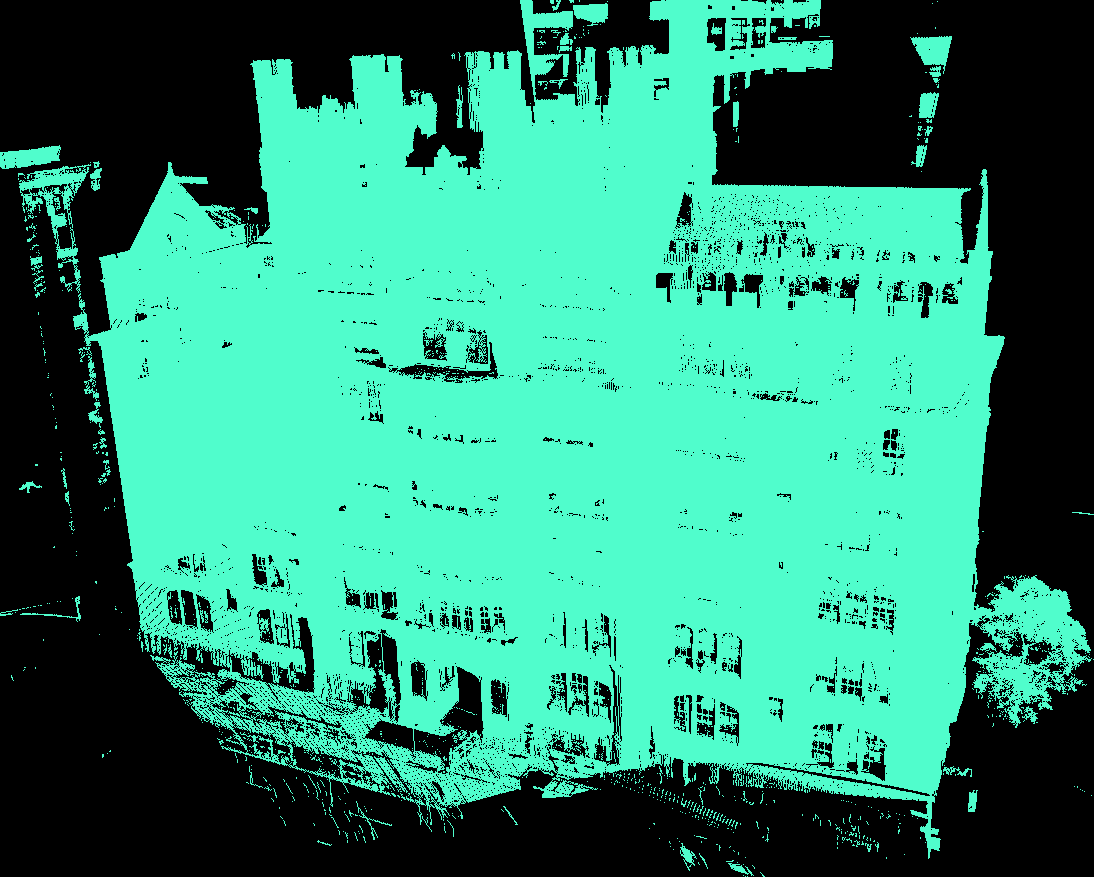
\includegraphics
        [width=0.5\textwidth]
	{figures/point_cloud.png}
  }
  \centering
  \subfloat[]{
    \label{fig_IR_2_DXF:b} %% label for first subfigure
    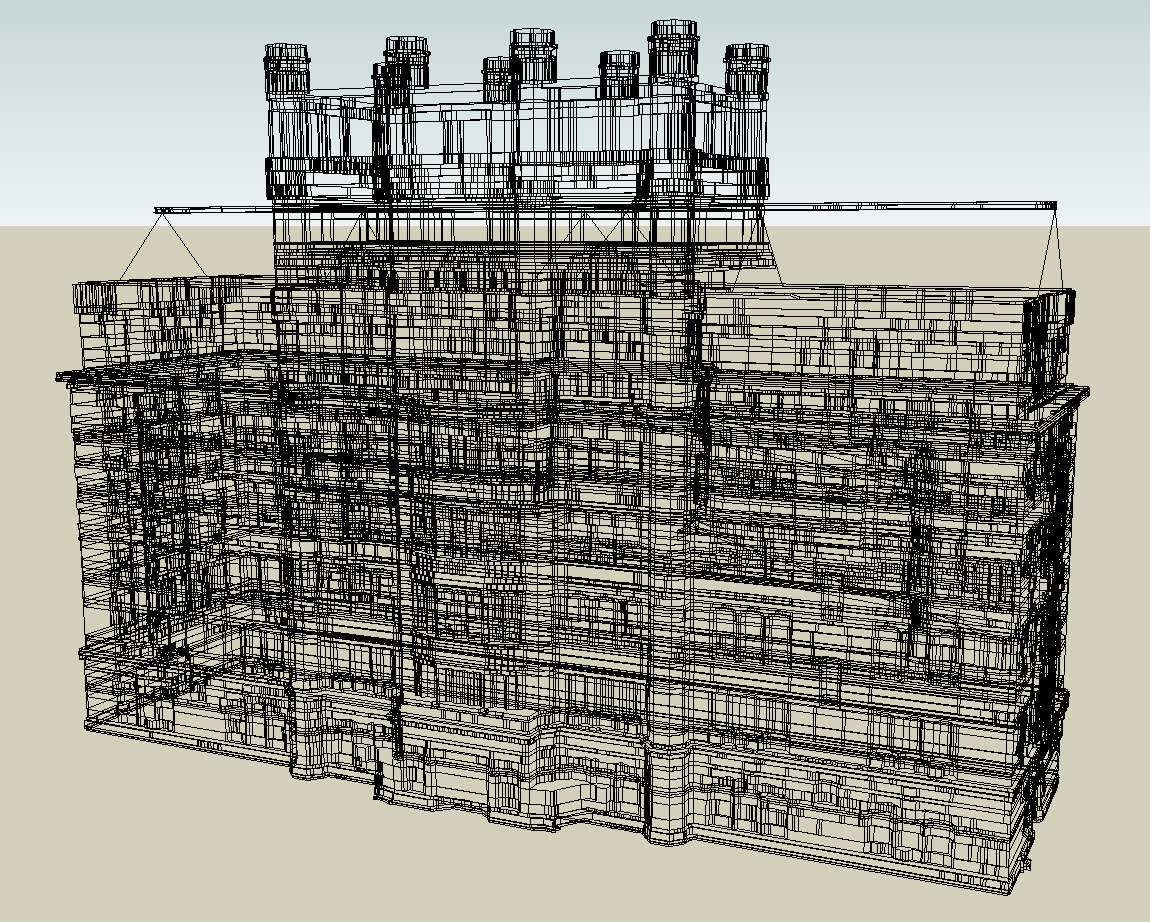
\includegraphics
        [width=0.5\textwidth]
	{figures/IR_skp_wireframe_1000_4_1_paper.png}
  }
  \vspace{.1in}
  \subfloat[]{
    \label{fig_IR_2_DXF:c} %% label for first subfigure
    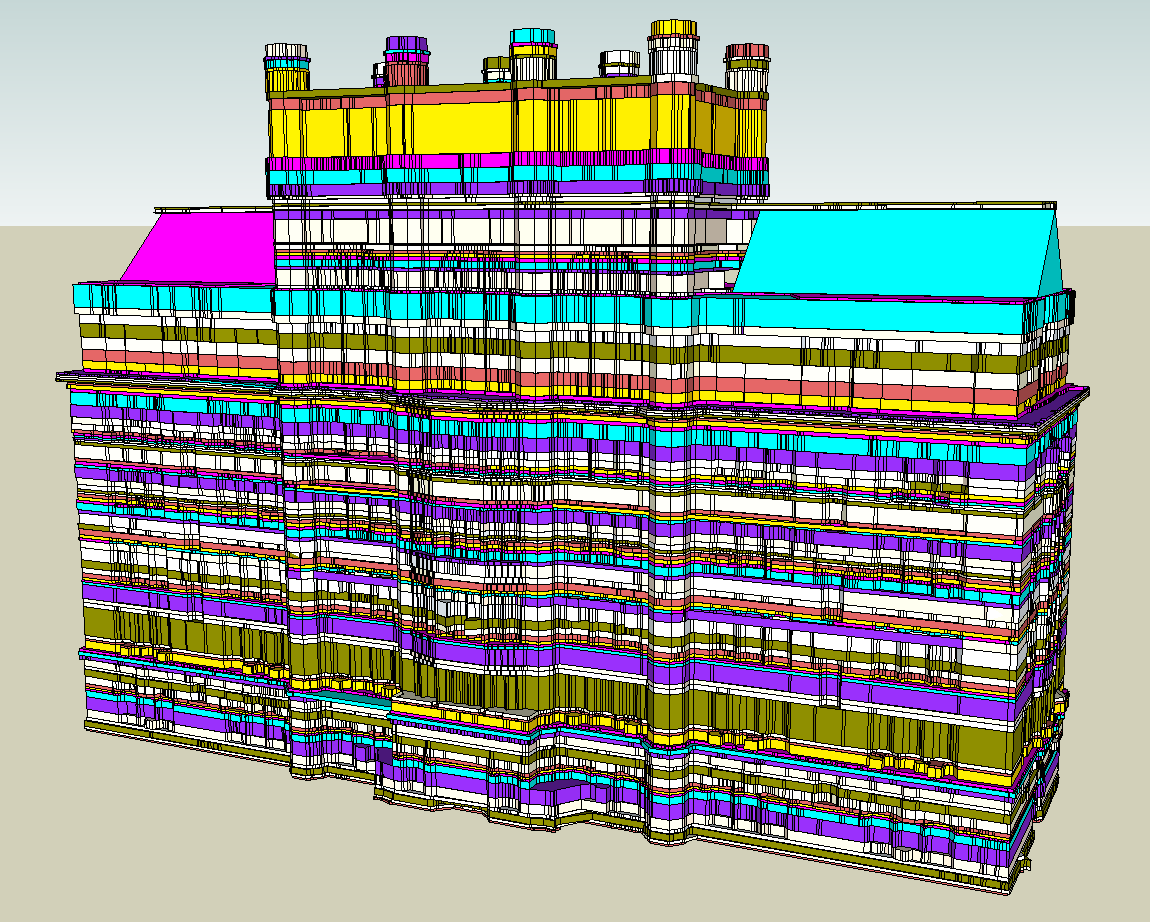
\includegraphics
        [width=0.5\textwidth]
	{figures/IR_skp_color_face_1000_4_1_paper.png}
  }
  \centering
  \subfloat[]{
    \label{fig_IR_2_DXF:d} %% label for first subfigure
    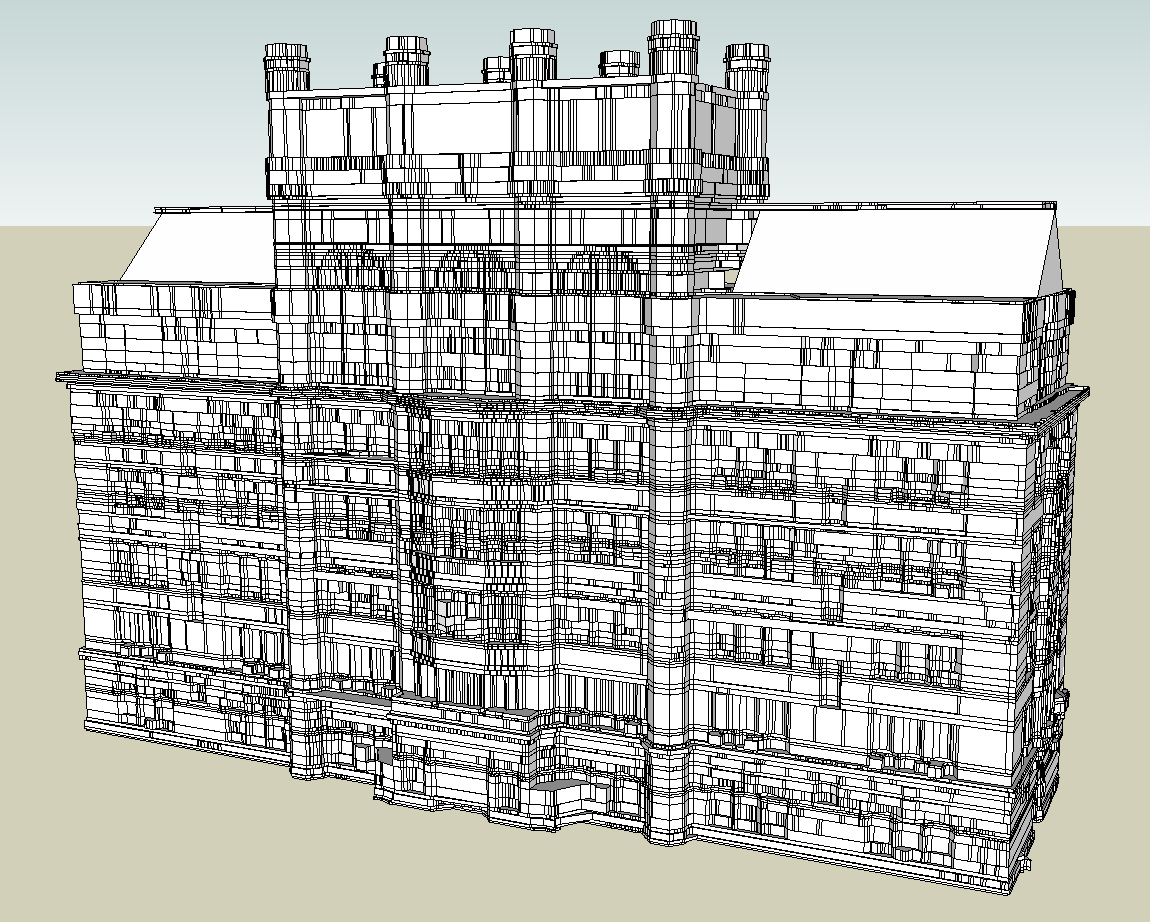
\includegraphics
        [width=0.5\textwidth]
	{figures/IR_skp_face_1000_4_1_paper.png}
  }
  \caption{ 3D point cloud and its reconstructed model of a building.
(a) A snapshot of the registered multiple scanning 3D point cloud data.
(b) wire-frame model of the building.
(c) colored layer model of the building.
(d) white face model of the building.}
  \label{fig_IR_2_DXF}
\end{figure}
%%% End of Figure


%%%%%%%%%%%%%%%%%%%%%%%%%%%%%%%%
%%%%%% Related Work    %%%%%%%%%
%%%%%%%%%%%%%%%%%%%%%%%%%%%%%%%%
%\section{Related Work}

% Refer to the following questions for writting.
% In \cite{RE_TOGSH}, what's been done, what approaches are proposed, what's the prons and cons.

There has been a lot of related work on 3D reconstruction research community.
In \cite{DP_OWYC}, Or et al. proposed a 3D building reconstruction from a 2D floorplan image.
With the help of 2D
floorplan image, both the interior and exterior of a building are reconstructed accordingly.
However, the unavailability of 2D floor plan makes this approach not applicable to most applications,
including our project.

Procedural modeling of buildings in \cite{PMB_MWH, PMB_WWS, PMB_PM} is proposed to automatically
generate buildings and streets of a city by using an effective description language. The strength
of the language is that it can generate a huge number of buildings and streets for a city quickly
and beautifully. This is particular useful for gaming or other computer graphics applications.
However, the parameters used to generate the buildings are randomly generated, which means the city
generated with these buildings and streets is not any existed city but a virtualized one.
In order to truthfully represent an existed building, one has to manually specify the parameters of the building,
which is very tedious and expensive. Our goal is to automatically infer the parameters for a building and therefore
reproduce the building quickly using the procedural modeling language described above.

Essentially, this inference process is a reverse engineering of computer graphics
\cite{RE_Fisher, RE_CLF, RE_CD}. Range data reverse
engineering has been applied in numerous research areas, such as computer-aided design (CAD),
computer vision, architecture modeling and medical image processing, etc.
In \cite{RE_TOGSH}, Thompson et al. made use of the manufacturing features as prior knowledge to
infer the 3D structure of the mechanical parts. Their method benefits from the domain knowledge
that most of the mechanical parts consist of predefined structures, such as holes, bosses, grooves, etc.
Our work is partially motivated by this idea, which also incorporates some prior knowledge on
the man-made building for further inference. However, their method is based on the assumption
that the input 3D data is of high signal-to-noise (SNR) ratio, which makes their approach not
applicable to those applications with low SNR and even incomplete data.

Medical image processing techniques are usually dealing with low SNR data.
There has been a lot of work on the medical 3D image reconstruction as in
\cite{MIR_FJS, MIR_BMMNB, MIR_KL, MIR_SKJ, MIR_SMHC, MIR_BVC}.
The basic ideas behind these approaches
are 3D reconstruction from sliced or histologic images using interpolation techniques.
The statistical inference are also intensively used to infer the low SNR images. For example,
In \cite{MIR_FJS}, Sigworth tried to deal with low SNR image data using maximum-likehood approach.
Because most of the statistical processes are computational intensity,
these approaches usually are heavy-duty approaches in order to obtain accurate, high resolution models.

An efficient way to reconstruct 3D model from range data is to project the data into 2D cross-section
or sliced images. This can avoid the direct computation on 3D data, which is time consuming and
computational complex. After the slicing, the image registration or similarity measure
\cite{IR_Brown,IR_ZF,RE_WWLZ} can be used to group or cluster the sliced images.
%The similarity measure can be divided into two basic research methods: area based method and feature based
%methods. The area based methods are computational efficient but they usually can only be applied on
%binary or gray-scale images. The second one is computational complex but more powerful and can be applied
%to images obtained using different sensors, such as multi-modal image registration.
And each clustered images can be represented using a \emph{key} image which usually shows the important
or salient structure of a building.

To generate the 3D model of a building, all these key raster images need to be vectorized to
represent the silhouette or boundary of the building. Couple of raster image vectorization approaches are
proposed in \cite{DP_AAKMT, DP_DP, DP_WM}. The Douglas-Peucker
algorithm tried to connect all the existed points to form a polygon. Although the implementation of
this approach is very efficient with the improvement in \cite{DP_HS},  this method cannot
handle the case where some extra interior points are existed as some outlier data.
To tackle this issue, Medeiros et al. \cite{BPA_MVL} applied ball-pivot algorithm (BPA)
\cite{BPA_BMRS}, which was original proposed on 3D point cloud data, on the 2D image to obtain
vectorized boundary. The key parameter for BPA to work successfully is to find the right size of
the ball for pivoting. We have proposed an adaptive BPA algorithm to solve this problem.



%%%%%%%%%%%%%%%%%%%%%%%%%%%%%%%%
%%%%%%   METHODS  %%%%%%%%%%%%%%
%%%%%%%%%%%%%%%%%%%%%%%%%%%%%%%%
\ifthenelse{\equal{\twocol}{true}}{
%\newpage % TWO COLUMN VERSION
}{
\newpage % TWO COLUMN VERSION
}
\section{Research Plan and Methodologies}

Our goal is to reconstruct, in a light-weight manner, 3D models of buildings from the point cloud data.
%This research is important since it provides an automatic and light-weight way to represent 3D building
%and therefore opens the door for those applications, such as web-based 3D city navigation, gaming, etc.
%A good example is 3D city navigation, including Google Earth\textsuperscript{\texttrademark} and Microsoft
%Virtual Earth\textsuperscript{\texttrademark}.
The approach we proposed is based on the observation that each man-made building can be viewed as the combination
of two types of basic components: the \emph{extruded} and the \emph{tapered} components. Therefore, to reconstruct
a 3D model of a building from its point cloud, we need only to identify its extruded
and tapered sub components and model them separately.
The 3D model of the entire building can be generated by integrating all the models of the sub components.
The key problem here is to identify those extruded and tapered sub components.
%represent them in an efficient way for reconstruction.

\begin{figure}[htb]
  \centering
  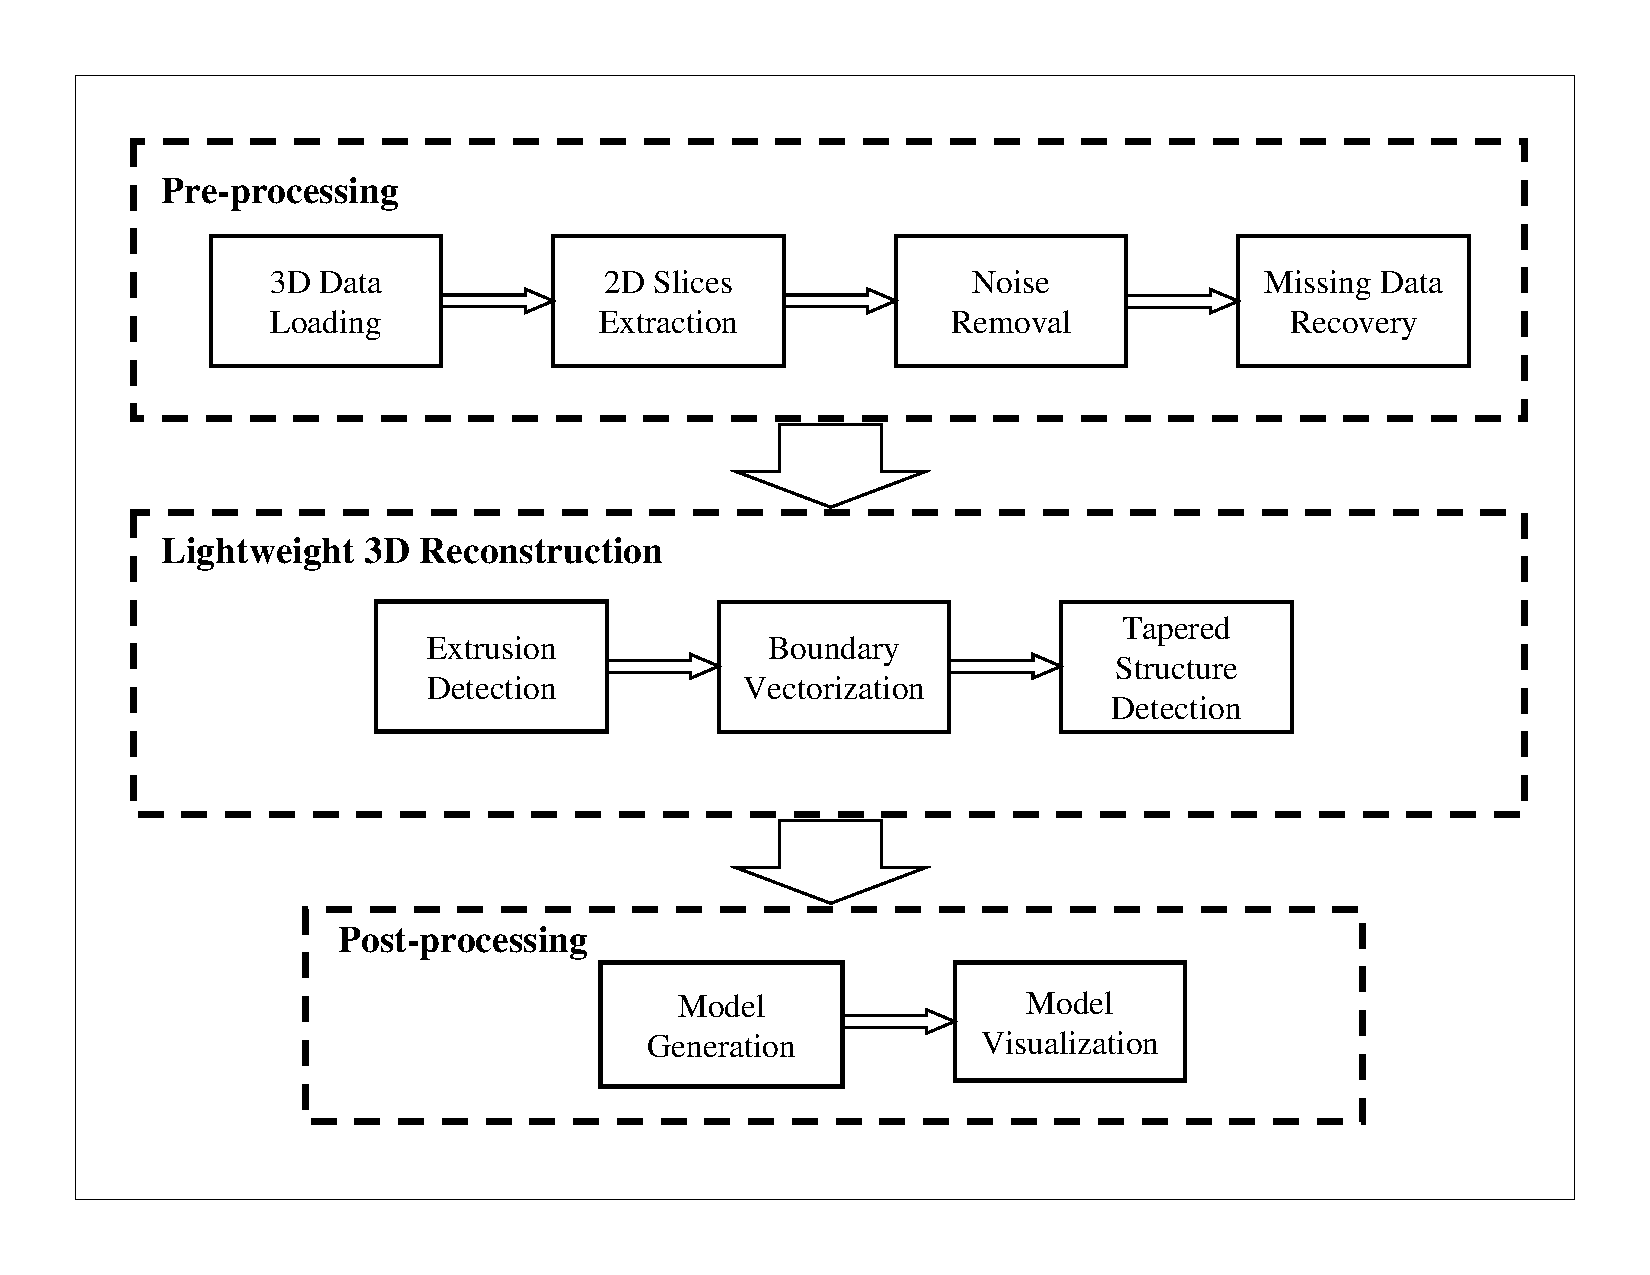
\includegraphics
      [width=\textwidth]
      {figures/flow.pdf}
      \caption{Flow graph for proposed approach}
      \label{fig_flow}
\end{figure}

The approach we proposed for 3D building reconstruction consists of
3 stages as shown in Figure \ref{fig_flow}.
First of all, the coordinates of the 3D point cloud stored in ascii format are loaded into memory.
%The most important
%information relies on the 3D coordinates with respect to an origin reference point.
%Because all data are refer to the same origin, this origin is useless for the further process.
%All data will be projected to the image coordinate of integer type from the 3D coordinate of float type with
%respect to a scale factor $\boldsymbol{S_0}$. The scale factor is adjustable by the users.
%All the following processes would use this scale factor $\boldsymbol{S_0}$ as a global reference factor.
%The 3D data can be projected along either $X$, $Y$ or $Z$ axis, with arbitrary number of slices.
%Without loss of the generality, let's assume the 3D point cloud is projected
%along the $Y$ axis with $N$ slices. Therefore, after data loading, we will obtain
%a series of images $\boldsymbol{I} = \{I_i, \; i = 0, \ldots, N\}$. This will be elaborated
%in the section \ref{sec_image_slicing}.
%Once the point cloud is projected to a serial of image slices $\boldsymbol{I}$, all the following steps
%can be carried out by using 2D image processing techniques.
Due to the occlusion and some special structures of the building, such as windows, the 3D data
is not complete and contains a lot of noise.
%existed in the 2D sliced images. In addition, the 3D point cloud is incomplete.
%For example, during the data collection, a corner of the building
%may be blocked by cars or trees nearby the building.
Therefore, the noise removal and missing data recovering are critical as a pre-processing stage to
generate the 3D model. To carry out light-weight process, the cleaned and enhanced 3D data
is projected to a serial of image slices. These will be addressed in the Section \ref{sec_mdr}.

The next stage of the approach is to carry out light-weight
3D modeling on the enhanced sliced images. As mentioned before, the goal is to reconstruct the 3D
model from the point cloud based on the extruded and tapered
components. Key slices detection will partition the whole point cloud data into some
basic extruded and tapered sub-components. After this, boundary vectorization for the raster
image will be conducted on the key images. Section \ref{sec_ksd} and
Section \ref{sec_BPA} will describe the algorithms and implementations on the key slices
detection and boundary vectorization.

%%%THESIS%%%
%Essentially, two adjacent key slices identify the extruded structure between this interval of
%the building. However, for tapered structure inference, it is not so straight-forward. First of all,
%a group of detected key slices may belong to the same tapered structure. We should be able
%to cluster these slices to the same structure. Usually to completely define a tapered structure,
%we only need to identify the bottom and top key slice of it. However, for those complicated
%tapered structure, special treatments are required for inference. Section \ref{sec_tsd} will address
%these problems.

To efficiently store these geometry structures and later on deliver and visualize the 3D
model, we adopted a simple intermediate representation. This will also allow us to convert
our internal model to any 3D model format easily.
Once all the above steps are completed, a 3D building model is reconstructed
from its range data. Figure \ref{fig_IR_2_DXF}\subref{fig_IR_2_DXF:b}-\ref{fig_IR_2_DXF}\subref{fig_IR_2_DXF:d}
shows an example of a 3D reconstructed model using Google SketchUp\textsuperscript{\texttrademark}. They
are represented with wire-frame, color face and regular face, respectively.

%%%%%%%%%%%%%%%%%%%%%%%%%%%%%%%%
%%%%%%   PREPRCESSING  %%%%%%%%%
%%%%%%%%%%%%%%%%%%%%%%%%%%%%%%%%
\subsection{3D Point Cloud Preprocessing}
\label{sec_prep}
Due to occlusion and some special structures, the point cloud collected by the
laser-range scanner \cite{RDP_LRS} contains noise and incomplete data.
%Therefore it is inappropriate to apply these data to any techniques directly.
In addition, computing on 3D data directly is time consuming and computational complex.
%difficult.Based on the above observations,
To tackle these issues, we carried out pre-processing on 3D point cloud data to remove noise,
recover the missing data and project the 3D data into a series of 2D cross-section images
for later model reconstruction.

\subsubsection{Noise Removal and Missing Data Recovering}
\label{sec_mdr}
There are two types of noise around the real 3D data. On the one hand, the exterior noise is due to objects
which block the laser beam of the scanner from hitting on the building behind them.
These noise data usually reflects these objects themselves, such as trees, human beings etc.
On the other hand, the interior noise is usually due to windows through which the laser beam went
and was reflected by the objects inside the building.
As a naive but effective way for noise removal, the interior and exterior 3D bounding boxes
are used to separate the real data from the noise. Only those data which stay between these two bounding boxes
are kept and others can be regarded as noise and can be discarded. Currently, the 3D bounding boxes
are chosen by users.

In addition to the noise, another main issue related to the input 3D data points is the incompletion.
%Because of the obstacle,  part of the building data blocked by surrounded objects is  missing, which largely
%affect the further process and lead to an incomplete 3D model.
We observed that most of the man-made buildings are self symmetry, which provides a
good hint for recovering the missing data. There are numerous papers on the symmetry computation
and measurement \cite{Sym_PSGRF, Sym_ZPA, Sym_TW, Sym_MGP}.
To simply the computation, we only need to infer the similarity on 2D sliced image.
%That is, the missing data inference happens after the image slicing introduced in the section
%\ref{sec_image_slicing}.
That is, before the similarity computation, we can project the 3D data into 2D images which will be introduced
in the Section \ref{sec_image_slicing}.
This simplification makes the symmetry computation much easier:
First of all, the input 3D point cloud data has already been rectified \cite{RDP_LSYGS},
which means we don't need to worry about the rotation for the data. Secondly, there is
no scaling issue for the data. In other words, only the translation needs to be considered here
for image symmetry computation.

Let $P(x,y)$ be a point on the original image $I$. Let $P'(x',y')$ be the reflected
point of $P$ with respect to a symmetry line $L$.
The symmetry computation equation for $L$ is as following:
\begin{equation}
L = \underset{x,y}{\operatorname{arg\,min}}\sum{d_{x,y}(P', I)}
\end{equation}
where the $d_{x,y}(P',I)$ is the distance between the self-reflected point $P'$ and its
nearest data point in the image $I$. The reflected point $P'$ of the original point $P$
is computed with respect to either a vertical line along $Y$ axis $Y = y$ or a
horizontal line along $X$ axis $X = x$. Therefore, the symmetry line $L$ is obtained
as the line with minimum summation error of the reflected data points.

%To speed up the computation, we can pre-compute a look-up table for the error
%function $d_{x,y}(P', I)$ based on the given image $I$. Once we have this look-up
%table, we can quickly obtain the error distance for each reflected point $P'$.


\subsubsection{Image Slicing}
\label{sec_image_slicing}
Slicing the 3D point data is to project the 3D point data into a series of 2D cross-section images.
We can choose any directions to project the 3D data. General speaking, projecting
data along axis $X$, $Y$ or $Z$ makes the task much easier.
In our laser scanning process, the axis $X$, $Y$ and $Z$ represent left-right, bottom-up and
face-inside directions,respectively.  However, the drawback of this process is some of
the 3D information is usually lost. For example, if we projected the data along $X$ axis, namely left-right
direction, the left-most and right-most sides of the building would be lost.
%Likewise, if we projected the data along $Z$ axis, namely inside-outside direction, the front-face side and
%the back side of the building would be lost.
Based on our observation, the best direction is along $Y$ axis, i.e., the bottom-up direction.
The reason is the top and bottom sides contain less structure information compared to other sides.
%Although the bottom and top side are missing, they are usually not visible
%for people. In addition, the top-most side is usually converging
%to a line or a small plane which will have no significant affect for the perception of the
%whole building.

To project the 3D data, a height interval, $\boldsymbol{\delta}$, is chosen for each projection.
$\boldsymbol{\delta}$ could be a fixed value, which means each sliced image is generated from
equal height range incrementally. $\boldsymbol{\delta}$ could also be a dynamic value, which
means we are projecting the similar structure of 3D data into the same image. To avoid working
on 3D data directly, a relative small and fixed $\boldsymbol{\delta}$ is chosen to generate 2D
cross-section images.
We model this as projecting any 3D data $\boldsymbol{P}(x,y,z), H_{lo} \leq y < H_{hi}$, in the
height range $[H_{lo}, H_{hi})$ onto a 2D image.

We use the following transformation $\boldsymbol{T_0}$ to get the 2D image:

%%% This is 3D line fitting equation.
\begin{equation}\label{eq_image_slicing}
%Vx' = \frac{\sum_{i}x_i*\sum_{i}z_i - N*\sum_{i}(x_i*z_i)}{\sum_{i}z_i*\sum_{i}z_i - N*\sum_{i}z_i^2}
\left\{ \begin{array}{l}
x^{2D} = \omega * (x^{3D}_i - X_{MIN}) \\
y^{2D} = \omega * (z^{3D}_i - Z_{MIN})
\end{array}\right.
\end{equation}
where, $\omega = W/(X_{MIN} - X_{MAX})$, $W$ is the image width,
the [$X_{MIN}$, $X_{MAX}$], and [$Z_{MIN}$, $Z_{MAX}$] pairs define the 3D bounding box, which
can be obtained through user input.
%The purpose of 3D bounding box is to rule out any noise data \emph{outside} of the box.
%For a building, those noise could be introduced by objects
%close to target building, such as trees, lamp posts, traffic signs or nearby buildings, etc.

%%% \textcolor{red}{ Description with BOX FILTER? }
%%% This is not exactly as BOX FILTER.



%%%%%%%%%%%%%%%%%%%%%%%%%%%%%%%%
%%%%%%   3D Reconstruct  %%%%%%%
%%%%%%%%%%%%%%%%%%%%%%%%%%%%%%%%
\subsection{Light-weight 3D Reconstruction}
\label{sec_reconst}
After the pre-processing, the noisy and incomplete point cloud data has been enhanced
and sliced into a series of 2D images using the transformation $\boldsymbol{T_0}$ defined
in the equation \ref{eq_image_slicing}.
%And hence the 3D reconstruction problem is converted
%to a 2D image processing problem.
Because we chose a relative small height interval $\boldsymbol{\delta}$
to equally slice the 3D data points in order to keep the structural details, a lot of
redundant and similar slices are generated. The next step is to cluster these sliced
images and compute the vectorization for the key slices for model reconstruction.
%The series of images $\boldsymbol{I}$ need to be clustered
%to keep only those key slices. In addition, the boundaries of these key images need to
%be vectorized. We have developed some light-weight techniques to accomplish these tasks.

\subsubsection{Key Slices Detection}
\label{sec_ksd}
An intuitive way for key slice detection is to compute the similarity between the sliced images.
In other words, the sliced images are clustered into different groups based on the similarity among them.
There are two mainly research methods for similarity measurement of 2D images: area based method and feature based
methods. The area based methods are computational efficient but they usually can only be applied on
binary or gray-scale images. The feature based one is computational complex but more powerful and can be applied
to images obtained using different sensors, such as multi-modal image registration.
% read similarity measure papers.
Because our goal is to develop light-weight efficient algorithm for model reconstruction, plus
the input for similarity measure is pure binary images, the area based method is adopted for our approach.
%%%THESIS%%%
%The classical measure for area based method is the normalized cross
%correlation \cite{DIP_Pratt}:
%\begin{equation*}
%CC(i,j) = \frac{\sum_W(W - E(W))(I_{(i,j)}-E(I_{(i,j)}))}
%{\sqrt{\sum_W(W - E(W))^2}\sqrt{\sum_{I_{(i,j)}}(I_{(i,j)} - E(I_{(i,j)}))^2}}
%\end{equation*}
%where $W$ is an image mask, $E(W)$ is the mean of the mask's pixels, and $E(I_{(i,j)})$
%is the mean of the image pixels covered by the mask $W$.
%However, this method is very time consuming and is a local window-based approach,
%which could not capture the global relations between images. Therefore, we proposed a
%light-weighted global and efficient key image detection approach based on Hausdorff distance \cite{IR_HKR}
%and curvatures computation.

For 3D building modeling, we are only interested in the boundary or silhouette of building.
Therefore, an image sweeping process is carried out for sliced images to obtain the boundary pixels
of each sliced layer. To measure the similarity of these boundary images, we adopted the Hausdorff
distance as the criterion for comparison.
\\
\\
\textbf{Hausdorff Distance}
\\
\\
Let $P_r(x_r, y_r)$ be a data point in a reference image $I_r$. Let $P_i(x_i, y_i)$ be a data point
in a new observed image $I$. The Hausdorff distance of the image $I$ to the reference image $I_r$ is defined
as following:
\begin{equation} \label{eq.hd}
d_H(I, I_r) = \sum_{i=0}^Nd_{min}(P_i, I_r)
\end{equation}
where, $d_{min}(P_i, I_r)$ is the minimum distance from a data point $P_i$ in the image $I$
to the reference image $I_r$. Alternatively, we can also define the Hausdorff distance,
$d_H(I_r, I)$, of the reference image $I_r$ to a new image $I$, using the equation \ref{eq.hd}.
%\begin{equation*}
%d_H(I_r, I) = \sum_{i=0}^Nd_{min}(P_{ri}, I)
%\end{equation*}
These two distances are usually not equivalent to each other. As a rule of
thumb, one can choose the $d_{HD} = \text{MAX}\{d_H(I, I_r), d_H(I_r, I)\}$ as the Hausdorff distance.
To compute the key slices, a threshold $\tau_{d}$ is used for the Hausdorff distance $d_{HD}$.
If $d_{HD} < \tau_{d}$, the two images $I$ and $I_r$ are treated as similar to each other. Otherwise,
a key sliced image is found and the $I_r$ is updated with $I$, the new key sliced image.

%%% THESIS
%To simply the computation, we adopted the manhattan distance for computation of $d(P_i, I_r)$.
%The Hausdorff distance therefore is the summation of the minimum distance for
%$N$ data points, $P_i$, in new image $I$ to the data points $P_r$ in reference image $I_r$.
%In addition to the Hausdorff distance based method, we also incorporate curvature
%information to avoid missing any salient structures for reconstruction.
The accuracy of the Hausdorff distance based key slices detection is mainly depend on the threshold $\tau_d$.
The smaller $\tau_d$ is, the more accurate the final model will be. Generally speaking, the more accurate the
model is, the more time and space are needed to compute and store the model. Therefore, for web-based
applications, there is a trade-off between the model accuracy and time and space efficiency.
This lead to an issue that some key slices or salient feature may be lost in the web-based application where
the threshold $\tau_d$ is relative large in order to keep the time and space efficiency.
To conquer this problem, we also use the curvature computation as a complementary method for the key slices detection.
\\
\\
\textbf{Curvatures Computation}
\\
\\
This idea is based on the observation that the key slices are generally located at
the places where the curvature of the orthogonal direction changes as shown in Figure
\ref{HT_BPA_Curvature}\subref{HT_BPA_Curvature:a}. Therefore,
instead of computing the difference between two images directly, we can compute the
curvature in the orthogonal direction, and map those places where the curvature changes
back to the key slice locations.

\begin{figure}[htbp]
  \centering
  \subfloat[]{
    \label{HT_BPA_Curvature:a} %% label for first subfigure
    \fbox{
      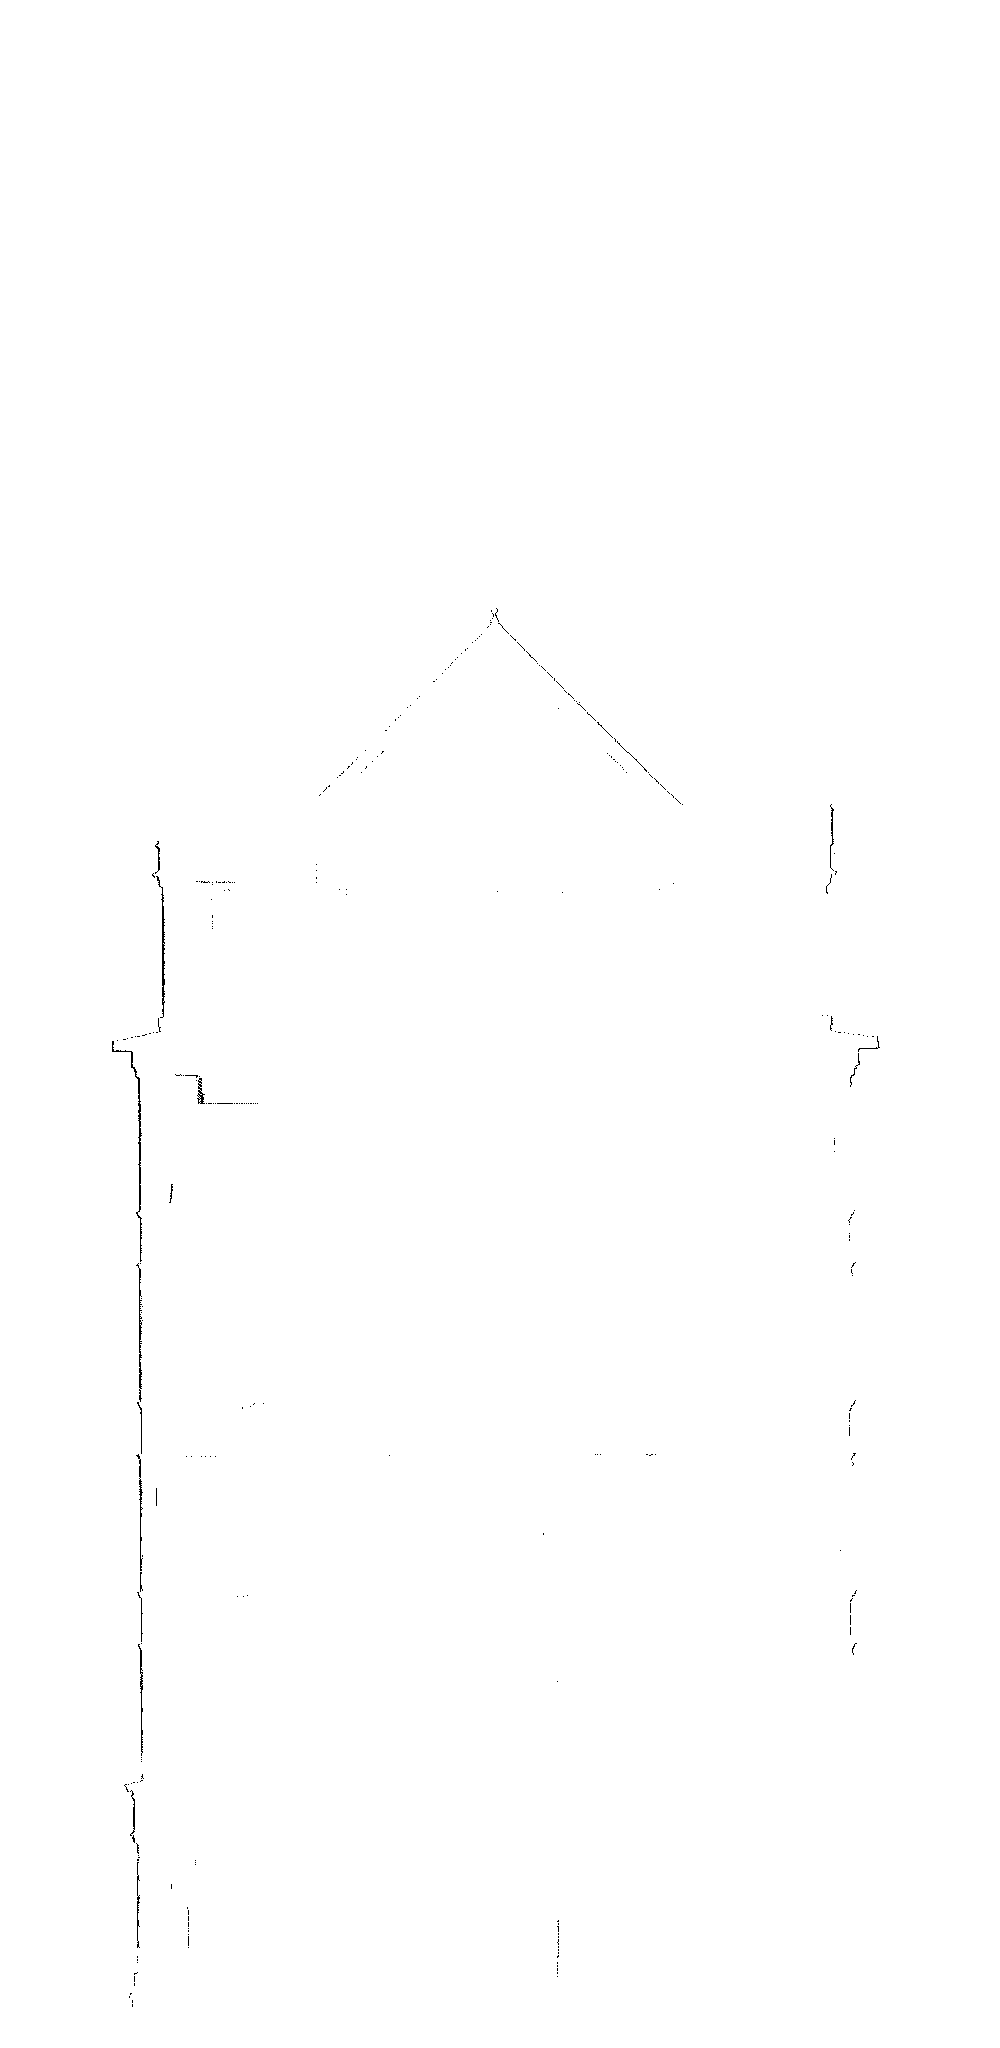
\includegraphics
	  [scale=0.25]
	  {figures/image_slice_1024_392_0820.png}
    }
  }
  \hspace{.5in}
  \subfloat[]{
    \label{HT_BPA_Curvature:b} %% label for second subfigure
    \fbox{
      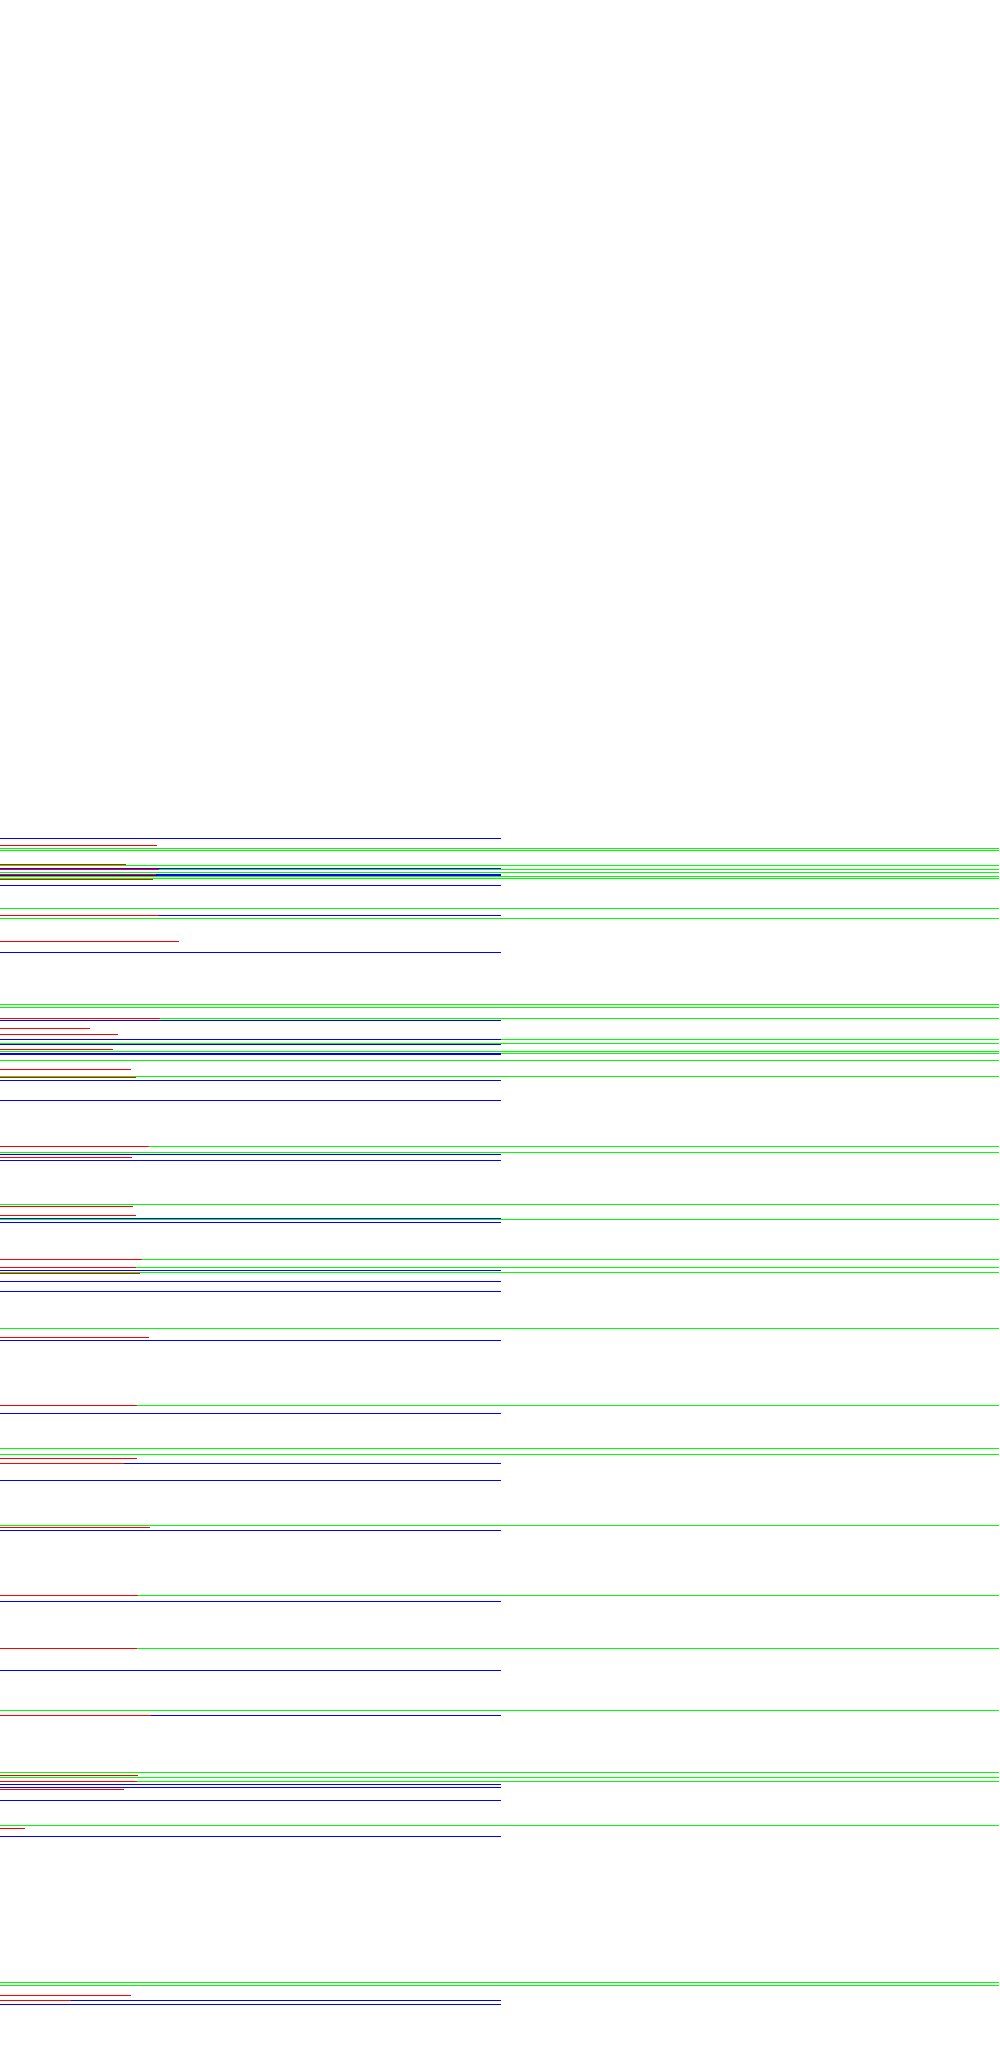
\includegraphics
	  [scale=0.25]
	  {figures/curvature_center_lines.png}
    }
  }
  \caption{ Curvature based key slice detection. (a) A slice image from the orthogonal direction.
(b) The average curvatures detected by a series of sliced image. }
  \label{HT_BPA_Curvature}
\end{figure}

To compute the curvature, we first apply the image slicing algorithm described in Section
\ref{sec_image_slicing}
to obtain a series of sliced images in the orthogonal direction. After that, we applied
ball-pivot algorithm described in Section \ref{sec_BPA} to vectorize the boundary for each
sliced image. We located those curvatures that appear in most of the sliced images as the
places where key slices are found as shown in Figure \ref{HT_BPA_Curvature}\subref{HT_BPA_Curvature:b}, where the red lines
indicated location of the center of the curvature, the blue and green lines indicate the
entering and exiting of the curvature structures. The combination of Hausdorff distance measurement
and curvature inference will guarantee that the salient structures of a building would be
preserved as well as the time and space efficiency for web-based applications.

\subsubsection{Boundary Vectorization of Raster Image}
After the key slices detection, $N_K$ key sliced images could be identified from the total $N_A$ sliced images.
Depend on the threshold $\tau_{d}$, $N_K$ is usually about 1 - 2 order smaller than $N_A$,
e.g., $N_K/N_A$ is 0.06 when $\tau_d$ = 4.0 for the example in Figure \ref{fig_IR_2_DXF}\subref{fig_IR_2_DXF:a}.
 Once we obtained these $N_K$ key sliced images, the next step is to vectorize these raster images for modeling.
%Because the goal is to model the silhouette of a building, we are only interested
%in the boundary of the raster images.

%%%THESIS%%%
%To vectorize the boundary of a binary image, Douglas-Peucker algorithm may be used to connect
%the pixels to form a polygon. Although the implementation of
%this approach is very efficient with the improvement in \cite{DP_HS},  this method
%is not desired for our requirement. The reason is because it tried to connect all the existed points,
%which cannot handle the case where extra points are usually existed as outlier data except
%the regular boundary data points.
%%%THESIS%%%

As we mentioned earlier, because of missing data which produces gaps between structures, it
is generally hard to determine an appropriate radius, $r$, of the pivoting ball in advance.
To solve this problem, a coarse-to-fine, adaptive ball-pivot algorithm is proposed.
The basic idea is to start with a relative big $r$ ( ensure the gap will be covered by the ball of radius $r$) as
a coarse step for the initial BPA to guarantee that the ball will travel all boundary data before
turning back or reaching any existed boundary points. After this, a refinement process
is applied on the obtained points to get more accurate results with smaller $r$.
The refinement will stop when $r$ is reduced to be less or equal to the threshold $\tau_r$.
\\
\\
\textbf{Ball-Pivot Algorithm}
\label{sec_BPA}
%%%THESIS%%% Here, the speeding up of the BPA algorithm should also be described in thesis.
\\
\\
%We applied 3D ball-pivot algorithm on 2D binary image to
%get the vectorized boundary. Since we are working on 2D image, we make the words ``ball'' and ``circle''
%interchangeable in the following description.
Ball-pivot algorithm which was original proposed by Bernardini et al. in \cite{BPA_BMRS} is an
efficient technique for 3D range data surface reconstruction. Because of its simplicity and efficiency,
we apply this algorithm on 2D image for boundary vectorization. The basic idea of the BPA algorithm is
shown in Figure \ref{fig_BPA}(a): pivot a ball or a circle on the data point, mark those points (in red)
which are touched by the ball. Keep doing the pivoting process until the ball could not touch any new points.
Although the basic idea is straight-forward, the implementation of BPA is not a trivial work.
A bad implementation has a significant impact on the efficiency and effective of the algorithm.
%%%THESIS
%
%Our implementation is as follows. Let $r$ and $C_0$ be the radius and center of the circle $C$
%to be used to pivot on the data point. To avoid the image boundary computation issue, we first pad the
%boundary of the original image with the length of $2r$, the diameter of the circle. Certainly,
%after the process is done, the padded image will be cropped back to the original size.
%
%The next step is to identify a starting set
%$\boldsymbol{S} = (P_0, \overrightarrow{\boldsymbol{R}})$, where
%$P_0$ is a point on which the circle $C$ stands and $\overrightarrow{\boldsymbol{R}}$ is the
%direction to which $\overrightarrow{P_0C_0}$ points. A good starting set is the one
%that the body of the circle $C$ will not touch any other points except $P_0$ in the image.
%Our strategy for finding a good starting set $\boldsymbol{S}$ is to scan from a side,
%e.g. left side, column by column and store the first data point $P_{0i}$ for column $i$.
%And then check for each $P_{0i}$, if it is sitting in almost the same location as its neighbors,
%we choose it as a possible starting point $P_0$. To validate $P_{0i}$, we
%try to put the circle on $P_{0i}$ with $\overrightarrow{P_{0i}C_0}$ parallel to
%the scanning direction, i.e., horizontal in this case. If the body of $C$ overlaps
%only the $P_{0i}$, namely it doesn't touch or cover any other data point, $P_{0i}$
%is chosen as $P_0$ in $\boldsymbol{S}$. Otherwise, we repeat the above steps until
%a good starting set is found. The intuition behind the strategy is to make sure
%the starting circle is sitting on a ``clear'' place, which is good for the following pivoting.
%
%%%%THESIS%%% Put a algorithm table here
%%%%THESIS%%% Speed up for various angle.
%
%%%% for writing, we should do another way around, opposite way %%%
%Once the starting set $\boldsymbol{S}$ is chose, we let the circle $C$ pivot around the starting
%point $P_0$ in a pre-defined direction, e.g., clock-wise direction with a small angle $\epsilon$.
%For each angle $\epsilon$ of pivoting, we check whether the region
%touched by the body of circle along the trajectory contains any new data point or not.
%If not, keep pivoting $C$ with the angle $\epsilon$ until it touches some new point set $S_P$.
%
%\begin{figure}[htbp]
%  \centering
%  \includegraphics
%      [width=0.6\textwidth]
%      {figures/BPA_rotate.pdf}
%      \caption{Ball pivot algorithm, $\theta_1$ is smaller than $\theta_2$, therefore
%	$P_1$ is selected as the next point. }
%      \label{fig_BPA_rotate}
%\end{figure}
%
%If $S_P$ only contains one point, it is trivial to add this point and
%its direction in the boundary point set, $\boldsymbol{\Phi} = \{(P, \overrightarrow{\boldsymbol{R}})
%|(P, \overrightarrow{\boldsymbol{R}}) \in \boldsymbol{S} \} $.
%Here, $\boldsymbol{\Phi}$ is an ordered list of the $(P, \overrightarrow{\boldsymbol{R}})$.
%However, if $S_P$ contains more than one point, which means a few data points are touched by $C$
%simultaneously, we would have to identify the earliest touched one in $S_P$. This is to make sure
%that the out-most point is chose, i.e. boundary points.
%
%A simple way to get this info is to re-pivot the circle with a smaller angle, say $\epsilon/2$,
%and check if only one new data touched. Though it is straight-forward, the drawback
%of this method is obvious: it is hard to know what is the right smaller angle for adjust
%and it may still touch more than one data points without knowing the right angle.
%To tackle this issue, we developed a reverse computation to compare the angles needed by $C$ to
%touch the points during pivoting. The smaller the angle is, the earlier the point will be
%touched. This is depicted in Figure \ref{fig_BPA_rotate}. The smaller dotted black circle
%is pivoting around the point $P_0$, and the whole region can be touched by the circle is
%illustrated in the bigger black circle. Data points $P_1$ and $P_2$ are touched after
%the pivoting angle of $\theta_1$ and $\theta_2$, respectively. It is obvious that $\theta_1$
%is smaller than $\theta_2$, hence, $P_1$ will be touched earlier than $P_2$ and is chosen
%as the possible next starting point.
%%%%THESIS%%%
%%%%The formula to compute the angle $\theta$ is:
%%%%\textcolor{red}{Equation here}.
%
%Each time when a new data point $P$ is chosen, it should be checked whether it belongs to existed
%boundary points in $\boldsymbol{\Phi}$ or not. If so, we would have done the initial BPA. Otherwise,
%we would have to update the two parameters, i.e., $P_0$ and  $\overrightarrow{\boldsymbol{R}}$ in
%$\boldsymbol{S}$, for next round pivoting.
\\
\\
%%%THESIS%%% \textcolor{red}{ Describe multiple boundary cases, like the 8 circles in slice for BPA. }
%%%THESIS%%% \textcolor{red}{ Describe speedup strategy here briefly and detailed in thesis. }
\textbf{The Refinement of the BPA}
\\
\\
% let's also describe the turning around case here for refinement? because for
% first basic BPA, there should be no turning around with big radius.
The output $\boldsymbol{\Phi}$, from the initial BPA, contains an ordered list of the boundary data
points $\boldsymbol{P}$ and their corresponding directions $\overrightarrow{\boldsymbol{R}}$ in which
the circle $C$ starts pivoting.
Because of the large radius $r$ in the initial BPA, $\boldsymbol{\Phi}$ is just a coarse representation
of the boundary and needs to be refined.

\begin{figure}[htbp]
  \centering
  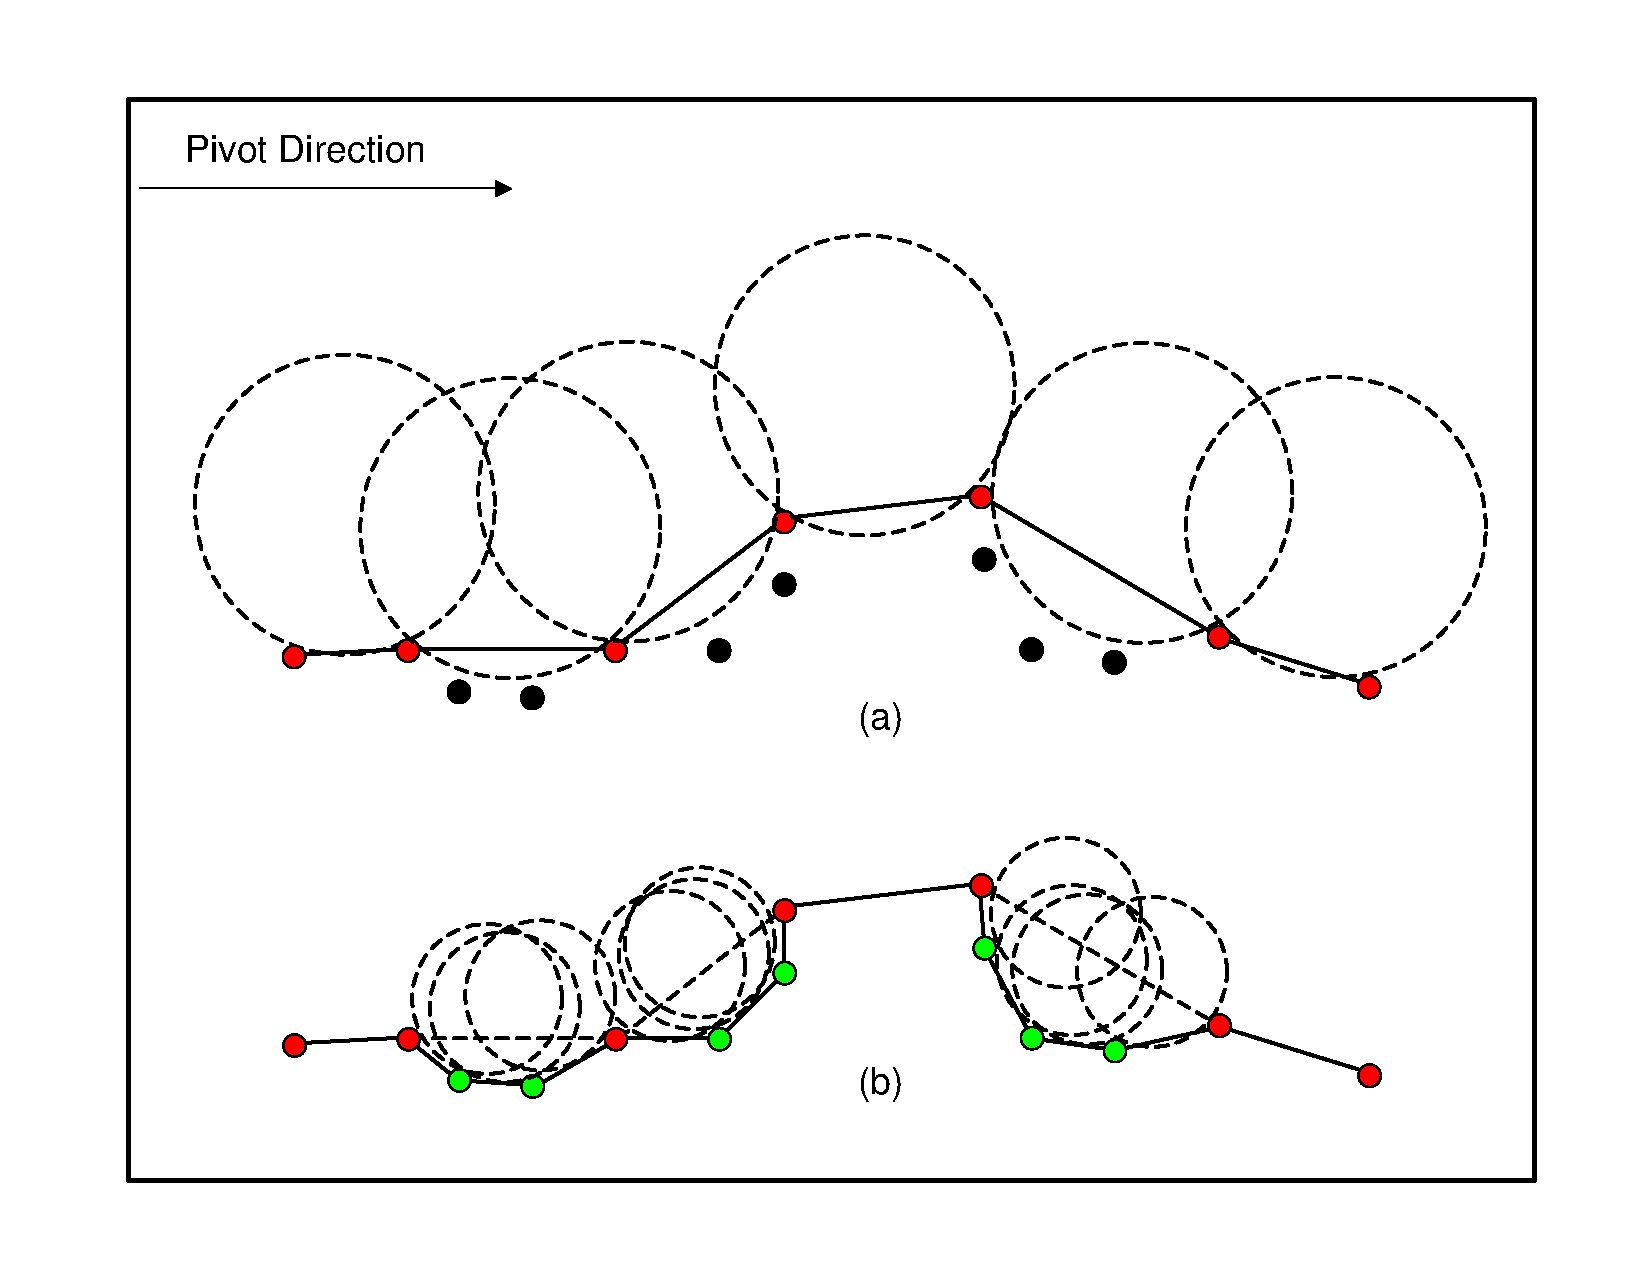
\includegraphics
      [width=0.8\textwidth]
      {figures/BPA.pdf}
      \caption{Ball pivot algorithm: (a) Initial pivoting with circle of radius 2$r$
	(b) Refinement process with circle of radius $r$.}
      \label{fig_BPA}
\end{figure}

%%%THESIS
%Because of missing data which produces gaps between structures,
%a big radius $r$ is chosen for the initial BPA to guarantee travel all boundary data before
%turning back and reaching exited boundary points in $\boldsymbol{\Phi}$.
%As expected, pivoting with this initial circle will produce a low resolution of the boundary.
%Therefore, to get detailed boundary or silhouette, a refinement stage based on the results of initial
%pivoting $\boldsymbol{\Phi}$ is needed.

The refinement algorithm is based on an iterative process with respect to the circle
radius $r$ as shown in Figure \ref{fig_BPA}(b). For each iteration, the radius of
the circle is reduced, e.g., $r' = r/2$. Then the length of the line segment formed by adjacent points
is checked, $\ell = \overline{P_0P_1}$, in $\boldsymbol{\Phi}$.
If this line is shorter than the new radius $r'$, it is ignored at this iteration. This is
because we can always leave short lines refinement to next rounds if needed.
If refinement is needed on $\ell$, the BPA algorithm with updated radius $r'$
is applied with parameters $\boldsymbol{S} = (P_0, \overrightarrow{\boldsymbol{R_0}})$.
That is, it takes the first point $P_0$ and its direction $\overrightarrow{\boldsymbol{R_0}}$
as input parameters. The BPA starts with the new circle $C'$ of radius $r'$, and
stops when either it reaches the end point $P_1$, or it turns back at a place where
the refinement ball size $r'$ is smaller than the gap between two data points.
If it reaches $P_1$, which means this pivoting process is valid, a new list
of ordered boundary points, $\boldsymbol{\Phi'}$, would be inserted into
$\boldsymbol{\Phi}$ between $(P_0, \overrightarrow{\boldsymbol{R_0}})$ and
$(P_1, \overrightarrow{\boldsymbol{R_1}})$.
%%%THESIS
%This makes $\boldsymbol{\Phi}$ a bigger
%ordered set of boundary points and is ready for possible further refinement.
On the other hand, If the circle $C'$ can not reach $P_1$, the new obtained
$\boldsymbol{\Phi'}$ would be discarded.
When the pivoting reaches the last point in the ordered list $\boldsymbol{\Phi}$,
this iteration with radius $r'$ ends.
The refinement algorithm repeats the iteration process until the new radius $r'$ is
smaller than the threshold $\tau_r = \omega * \tau_d$, where $\tau_d$ is the threshold for Hausdorff distance
and $\omega$ is a scale factor for the threshold $\tau_r$ with respect to $\tau_d$.
%%%THESIS
%Essentially, the BPA refinement process is similar to the initial one except that
%we have to take care of the turning-back case as well as different stop case (reached $P_1$).
%To detect the turning-back case, we can check
%the angle $\theta$ between the direction of a new detected data point $P$ and
%that of the previous detected one. If the angle is equal to or close to the 180 degree,
%it indicates that the circle is turning back and therefore we should stop the pivoting
%and discard the new list $\boldsymbol{\Phi'}$ detected during the BPA process.
%
%
%As a post-process stage, we can quickly simply the boundary by merge those adjacent data points
%sitting on the same line, i.e., with the same slope. This is a special treatment for those
%sliced images  with little noise and plenty of straight-line structures existed.
\\
\\
\textbf{The Integration of BPA and HT}
\\
\\
Although the adaptive BPA is a very efficient and straight-forward approach to vectorize
the boundary or silhouette of raster images, it is prone to the noise. This is illustrated
in Figure \ref{HT_BPA_figure}\subref{HT_BPA_figure:a}. As we can see, the upper part of the vectorized image
contains some bogus detailed structures which actually belong to the same line structure. In the
case where the outlier is not close enough to the real data, the result will be significantly
degraded. Based on the observation that most of the boundaries of the man-made building
are of line structures, we can improve the adaptive BPA results by incorporating the line
information.

\begin{figure}[htbp]
  \centering
  \subfloat[]{
    \label{HT_BPA_figure:a} %% label for first subfigure
    \fbox{
      \includegraphics
          %[angle=90, scale=0.25]
          [width=0.75\textwidth]
	  {figures/bbb_image_slice_1024_392_0533_refine_with_rad_1_and_merged.png}
    }
  }
  \vspace{.2in}
  \subfloat[]{
    \label{HT_BPA_figure:b} %% label for second subfigure
    \fbox{
      \includegraphics
          %[angle=90, scale=0.25]
          [width=0.75\textwidth]
	  {figures/bbb_image_slice_1024_392_0533_combine_HT_BPA_rad_32.png}
    }
  }
  \caption{ (a) a sliced image vectorization with adaptive BPA
(b) the combination of hough transform and BPA on the sliced image. }
  \label{HT_BPA_figure}
\end{figure}


%%% Adaptive Hough Transform %%%
%%\subsubsection{Adaptive Hough Transform}
%%%THESIS
%In order to effectively obtain the line information for a raster image, we proposed
%an adaptive hough transform (AHT) for line detection.
%The intuition behind the AHT is to make the HT more robust to non-perfect data set.
%Even though the sliced image has been applied noise removal, missing data recovering,
%there are still a moderate outlier data or missing data on the image. By doing AHT,
%the non-perfect data set has only limited impact on the line detection of the image $I$.
%
%The AHT is an iterative algorithm. The idea is to detect the longest line $L_0$ in
%each iteration in image $I$, and remove those data points sitting along $L_0$.
%By doing this, all the outlier data close to the long lines will be removed and
%the image $I$ is updated for the next round of processing. The longest line $L_0$
%is saved in a line set $\boldsymbol{L}$ for further process.
%By applying the same strategy on the updated image $I$, we can obtain a series of
%lines in $\boldsymbol{L}$ until there is no more data or the data is sparse enough
%in the image $I$. Here, the sparse means there is not enough data point sitting
%around any new detected line. This algorithm is illustrated in the Algorithm
%\ref{alg.AHT}.
%
%%%%%
%\begin{algorithm}
%\caption{The Adaptive Hough Transform Algorithm}
%\label{alg.AHT}
%\begin{algorithmic}[1]
%\Procedure {adaptive\_hough\_transform}{$I$, $\boldsymbol{L}$}
%\While {$true$}
%\State $[\rho, \theta] = hough\_transform(I, im\_h, im\_w)$
%\State $I = update\_image(I, \rho, \theta)$
%\State $\boldsymbol{L} = update\_line\_set(\rho, \theta)$
%\If {$num\_of\_data\_points(I) < \epsilon$}
%\State $break$
%\EndIf
%\EndWhile
%\EndProcedure
%\end{algorithmic}
%\end{algorithm}
%%%%

To combine the adaptive BPA with HT, we first apply our adaptive HT algorithm on the raster
image to obtain all lines $\boldsymbol{L}$ and sort them from the longest to the shortest one.
Generally speaking, the longer lines give more confidence on the line structure of the building.
For integration, we first apply dilation operation on $I$ using 8-connected kernel
%%%THESIS
%as shown below:
%\begin{equation*}
%A \oplus B = \{x \ |\ (\hat{B})_x \cap A \ne \phi \}
%\end{equation*}
%where $\hat{B}$ is the refection of $B$, i.e., $\hat{B} = \{x \ | \ x = -b, \quad \text{for} \; b \in B\}$,
%and $(B)_x$ denotes the translation of $B$ by $x$. Here, we defined B as an 8-connected kernel, $N_8$.
%%%THESIS
to get the dilation image, $I_d$. The next step is to measure how well the lines in
$\boldsymbol{L}$ match the data in $I_d$. This will determine whether a line in $\boldsymbol{L}$
should be used as a substitution or not.

If a line segment $L$ is found to be a good candidate, the next step is to find the corresponding part of the
BPA points in $\boldsymbol{\Phi}$ for substitution. To do this, we first compute the closest two points
$P_i$ and $P_j$ in $\boldsymbol{\Phi}$ to the two end points of $L$.
%its two end points, $E_0$ and
%$E_1$, are computed to replace part of the BPA points in $\boldsymbol{\Phi}$.
%The way is to find two closest BPA points with respect to $E_0$ and $E_1$.
General speaking, the points in $\boldsymbol{\Phi}$ represent a polygon and therefore form a circle layout, i.e.,
$\boldsymbol{P} = \{ P_0,P_1,\ldots ,P_{n-1}, P_0 \}$. Assume $i < j$, there are two possible choices to replace
the series of the points, which are
$\boldsymbol{P_1} = \{ P_i,P_{i+1},\ldots,P_{j-1}, P_j \}$, and
$\boldsymbol{P_2} = \{ P_j,P_{j+1},\ldots,P_{i-1}, P_i \}$.
To determine which one is correct, one can compare the distance, $D$, from the line $L$ to both
set of the points $\boldsymbol{P_1}$ and $\boldsymbol{P_2}$. The point set with smaller $D$ is
about to be substituted by the line $L$.
\begin{equation*}
D = \underset{\boldsymbol{P_1},\boldsymbol{P_2}}{\operatorname{arg\,min}}\sum{\lVert P_i - L \rVert}
\qquad P_i \in \boldsymbol{P_1} \ \text{or} \ P_i \in \boldsymbol{P_2}
\end{equation*}
where $\lVert P_i - L \rVert$ is the Euclidean distance from a point $P_i$ to the line $L$.

%%%%%%%%%%%%%%%%%%%%%%%%%%%%%%%%%%%%%%%
%%%% Let's describe this in thesis %%%%
%%%%%%%%%%%%%%%%%%%%%%%%%%%%%%%%%%%%%%%
%\subsubsection{The Implementation of Adaptive BPA}

%Describe the global threshold and settings?

\subsubsection{Tapered Structure Detection}
\label{sec_tsd}
After the key slices detection and vectorization, $N_K = \{I_{i}, i = 0, ..., K \}$ key slices are detected and
the silhouette of $N_K$ can be used to represent the whole building based on extrusion operation.
That is, the space between each pair of key slices, say $I_{i}$ and $I_{j}$, can be interpolated
by the lower key slice, e.g., $I_{i}$ in this case. This is valid because of the similarity between
the intermediate images and the key sliced image $I_{i}$. By modeling a building using this series
of key slices $N_K$, we can largely reduce the space needed to store a building and therefore
make the 3D web-based application, such as 3D city navigation applicable.

In addition to the extrusion operation, we can further improve the model and reduce the model size
based on the observation that part of key sliced images belong to the same tapered structure. This is
demonstrated in Figure \ref{fig_DXF_top}. Figure \ref{fig_DXF_top}\subref{fig_DXF_top:a} shows the roof structure
viewed from the top of the building with almost half of the key sliced images dedicated to represent
the roof structure. After applying the tapered structure inference, Figure \ref{fig_DXF_top}\subref{fig_DXF_top:b}
shows the improvement of the modeling. As we can see, the roof lines in Figure \ref{fig_DXF_top}\subref{fig_DXF_top:b}
are much more smooth and straight than those in Figure \ref{fig_DXF_top}\subref{fig_DXF_top:a}. In addition, the key slices
needed to represent the building are reduced almost half and so does the store space.

The difficulty of tapered structure inference depends on how complicate the part of a building
to be inferred is. Let's assume the height range for roof structure to be inferred
is $H_R = [H_{lo}, H_{hi}]$. If there is only a single unit with tapered structure existed
between $H_R$, it is simple and straight-forward to detect and infer this part.
%Namely, we only need to find the corresponding feature points between the bottom
%the top feature points.
However, for some complicated structures, such as a mixed layout
of tapered and extruded structure, some special treatment are needed to obtain
the desired results. Our approach is based on divide and conquer strategy:
the whole structure $\boldsymbol{U}$ is segmented
into independent sub-structures, $U_0, U_1, \ldots, U_N$. For any sub-structure $U_i$,
it contains only an independent structure, either a tapered or an extruded one. Once
each unit $U_i$ is inferred, the whole structure can be obtained by an union operation
of these sub-structures, i.e., $\boldsymbol{U} = \bigcup{U_i\{ i = 1,\ldots,N\}}$.

%%% Figure of the tapered template.
\begin{figure}[htbp]
  \centering
  \subfloat[]{
    \label{fig_DXF_top:a} %% label for first subfigure
    \includegraphics
        [width=0.8\textwidth]
%	{figures/BPA_250_top_crop.png}
	{figures/extrude_1.png}
  }
  \vspace{.5in}
  \subfloat[]{
    \label{fig_DXF_top:b} %% label for first subfigure
    \includegraphics
        [width=0.8\textwidth]
%	{figures/BPA_250_top1_crop.png}
	{figures/extrude_2.png}
  }
  \caption{  The top view of the 3D building. (a) without tapered structure. (b) with tapered structure }
  \label{fig_DXF_top}
\end{figure}
%%% End of Figure

Before segmentation, the potential height ranges $H_R$ containing the tapered structures should be computed.
This can be done by checking the frequency of the key sliced images.
The structure containing tapered sub-structures will show a high and even
distributed key sliced images. This is a very useful clue for $H_R$ detection.
For example, the roof structure of a building satisfies the above observation,
and the corresponding range of $H_R = [H_{lo}, H_{hi}]$ can be detected.

Once the potential height ranges $H_R$ in bottom-up direction ($Y$ axis) is obtained,
the next step is to segment the whole structure $\boldsymbol{U}$ between $H_R$ into
sub-structures, $U_i, \; i = 0,\ldots,N$. This is again done by similarity measurement of sliced images
in orthogonal directions. As before, the 3D data points following inside the range of $H_R$
are projected along both left-right ($X$ axis) and face-inside ($Z$ axis) directions.
Then the key slices detection is carried out based on Hausdorff distance similarity measurement for
both directions. These key slices will segment the structure in $H_R$ into sub units of $U_0, U_1, \ldots, U_N$.

%%%THESIS
%%% Figure of the tapered template.
%\begin{figure}[htbp]
%  \centering
%  \subfloat[]{
%    \label{TSD_fig_tapered_template:a} %% label for first subfigure
%    \fbox{
%      \includegraphics
%	  [scale=0.25]
%	  {figures/acc_template_lr.png}
%    }
%  }
%  \hspace{.5in}
%  \subfloat[]{
%    \label{TSD_fig_tapered_template:b} %% label for first subfigure
%    \fbox{
%      \includegraphics
%	  [scale=0.25]
%	  {figures/acc_template_face.png}
%    }
%  }
%  \caption{  The template for tapered structure. (a) left-right template. (b) face-inside template }
%  \label{TSD_fig_tapered_template}
%\end{figure}
%%% End of Figure

For each sub unit $U_i$, we have to know whether it represents an extruded or a tapered
structure. The method is to check in the key sliced image $I_k$ of $U_i$ whether there exists
a pattern where two lines intersect with some appropriate angle.
% as shown in Figure \ref{TSD_fig_tapered_template}.
If such a pattern exists in $I_k$, the
unit $U_i$ is marked as a tapered sub-structure. Otherwise, $U_i$ is marked as
an extruded sub-structure. If $U_i$ is an extruded unit, its silhouette from the
$Y$ axis is vectorized and is ready for the union operation to obtain $\boldsymbol{U}$.

On the other hand, if $U_i$ is a tapered unit, the bottom and top position have to be computed
so that it can be reconstructed. To do this, all line segments $\boldsymbol{L}$ in $U_i$
are computed using hough transform and the
%described in Algorithm \ref{alg.AHT}.
intersection point $P_0$ of $\boldsymbol{L}$ indicates
the top position of the tapered unit. The other end points $P_i$ of $\boldsymbol{L}$ are also computed
to infer the bottom shape and position.
%converging to $P_0$ in this tapered unit. Therefore, the bottom shape and position
%can be inferred from $P_i$. For example, in Figure
%\ref{TSD_fig_tapered_template}, we can see key sliced images of tapered
%units from both left-right direction as shown in Figure \ref{TSD_fig_tapered_template}\subref{TSD_fig_tapered_template:a} and
%face-inside direction as shown in Figure \ref{TSD_fig_tapered_template}\subref{TSD_fig_tapered_template:b}. Because the key sliced
%images represent extruded structures for a certain range, we can
%infer that the bottom structures are both rectangles for tapered units in Figure
%\ref{TSD_fig_tapered_template}. The four points of the rectangle are computed
%based on the starting and ending position of the unit as well as the end points
%$P_i$ in $\boldsymbol{L}$. Once all sub unit $U_i$ is reconstructed, the whole
%structure $\boldsymbol{U}$ can be modeled via union $U_0 \cup U_1 \cup \ldots
%\cup U_N$.

%%%THESIS
%The structure $\boldsymbol{U}$ together with its range information are saved
%in our intermediate representation (IR) and can be easily transformed to one of
%the standard 3D representation, such as DXF format.
%%%

%Although our method can only handle rectangle tapered structure at this point, it
%is good enough to process most of the man-made buildings with complex roof structure.
%Please note, for simple independent roof structure, it is trivial to infer any
%type of the tapered polygon bases.


%%%%%%%%%%%%%%%%%%%%%%%%%%%%%%%%
%%%%%%   3D OUTPUT       %%%%%%%
%%%%%%%%%%%%%%%%%%%%%%%%%%%%%%%%
\subsection{Preliminary Results}
\label{sec_IR_OUT}

%%%%%%%%%%%%%%%%%%%%%%%%%%%%%%%%
%%%%%%   Experimental Results%%%
%%%%%%%%%%%%%%%%%%%%%%%%%%%%%%%%

%%%THESIS
%The building shown in Figure \ref{fig_IR_2_DXF} suggests that the part below the big ledger
%can be basically viewed as an extruded structure. On the other hand, the top part of the building is
%a mixture of the extruded and tapered structure. Part of the bottom structure is missing because of
%the occlusion by another building right behind the modeling building during the data collection.

After  the extruded and tapered structures are computed and vectorized for 3D point cloud,  we can
some existed modeling language to represent the 3D point cloud, such as Generative Modeling Language (GML)
introduced in \cite{CTE_GML}. This representation is ready to be transformed to any 3D modeling format for visualization.
%%%THESIS
%However, for our special application,
%the GML is not efficient and therefore a light-weight representation is developed here
%to represent the building model based on the script language introduced in procedural
%modeling of buildings \cite{PMB_MWH}.
%%%

\subsubsection{Model Generation}

%%%THESIS
%Once the 3D point cloud is modeled and represented using the intermediate representation, it
%can be readily converted to any other representations for visualization or other applications.
%As an example, we will show how to
%convert the IR into DXF representation which is widely used in computer-aided
%design (CAD) and other applications.
%Essentially, the DXF representation keeps track of the 3D coordinates of geometry points
%with respect to a reference coordinate system. Therefore, to convert the IR to DXF, we only
In order to generate the final 3D model for visualization from its modeling language representation which basically stores
2D vectorized structures, we need to convert a point, $P(x,y)$, in 2D image coordinate back to its 3D real coordinate,
$P'(x,y,z)$. Here, $z$ is the depth coordinate. For all points in the same layer of boundary or
silhouette, they lay in the same planar and hence have the same value of $z$.

The equation for transforming $P$ back to $P'$ is a reverse transformation of $\boldsymbol{T_0}$
in the equation \ref{eq_image_slicing}:
\begin{equation}\label{eq_ir2dxf}
\left\{ \begin{array}{l}
x^{3D} = \{ [ x_1 + \omega * ( x_2 - x_1 ) ] + T_x \} * S_x \\
y^{3D} = \{ [ y_1 + \omega * ( y_2 - y_1 ) ] + T_y \} * S_y \\
z^{3D} = z^{3D}_0 + T_z
\end{array}\right.
\end{equation}
where $\omega$ is a scale factor for locate the point of the two end points.
%%%THESIS%%%
%%%\textcolor{red}{See figure ???}.
$T_x$, $T_y$ and $T_z$ are the translation of the 3D points on $X$, $Y$ and $Z$ axis,
respectively.  $S_x$ and $S_y$ is the scale factor on $X$ and $Y$ axis.

\subsubsection{Error Measurement}
To measure the error between a reconstructed 3D model and its original point cloud,
we first mapped the generated model back to the 3D point cloud coordinate system.
The error is measured as the distance from the sampled 3D cloud data to their closest model planes, which
is computed using the following formula:
\begin{equation}\label{eq_em}
E = \frac{1}{|X|}\sum_{x\in{X}}{d^2(x, M)}
\end{equation}
where $X$ is the set of 3D point cloud data. The distance
$d(x, M) = \text{min}_{p \in M}\lVert x - p \lVert$ is the minimum Euclidean distance from
a 3D point $x$ to its closest face $p$ of $M$.

\begin{table}[hbtp]
%\centering
%\subfloat[]{
%  \label{tab_em:a} %% label for first subfigure
%  \begin{tabular}[t]{||c||c|c|c||}
%    \hline
%    $\tau_r$ & Error & \# of faces & Model size (KB) \\
%    \hline \hline
%    64 & 3.65 & 8016 & 81\\
%    \hline	       		
%    32 & 2.83 & 10816 & 111\\
%    \hline	       		
%    16 & 2.20 & 14711 & 147\\
%    \hline	       		
%    8 & 1.69 & 20788 & 204\\
%    \hline	       		
%    4 & 1.38 & 27214 & 261\\
%    \hline	       		
%    2 & 1.30 & 33909 & 331\\
%    \hline	       		
%    1 & 1.29 & 33911 & 332\\
%    \hline
%%    \hline
%%    $\tau_r$ & Error & \# of faces \\
%%    \hline \hline
%%    64 & 4.69 & 8016 \\
%%    \hline
%%    32 & 3.84 & 10816 \\
%%    \hline
%%    16 & 3.15 & 14711 \\
%%    \hline
%%    8 & 2.58 & 20788 \\
%%    \hline
%%    4 & 2.29 & 27214 \\
%%    \hline
%%    2 & 2.23 & 33909 \\
%%    \hline
%%    1 & 2.22 & 33911 \\
%%    \hline
%  \end{tabular}
%}
%\hspace{.1in}
\centering
%\subfloat[]{
%  \label{tab_em:b} %% label for first subfigure
  \begin{tabular}[t]{||c||c|c|c||}
    \hline
    $\tau_{d}$ & Error & \# of faces & Size (KB) \\
    \hline \hline
    64 & 0.658 & 1471 & 15\\   %   64 & 9.63 & 1471 & 15\\ 
    \hline		      %   \hline		    
    32 & 0.294 & 3284 & 32\\   %   32 & 4.30 & 3284 & 32\\ 
    \hline		      %   \hline		    
    16 & 0.141 & 8574 & 86\\   %   16 & 2.06 & 8574 & 86\\ 
    \hline		      %   \hline		    
    8 & 0.131 & 13955 & 137\\  %   8 & 1.91 & 13955 & 137\\
    \hline		      %   \hline		    
    4 & 0.094 & 27214 & 261\\  %   4 & 1.38 & 27214 & 261\\
    \hline		      %   \hline		    
    2 & 0.088 & 31331 & 335\\  %   2 & 1.28 & 31331 & 335\\
    \hline		      %   \hline		    
    1 & 0.083 & 32187 & 337\\  %   1 & 1.21 & 32187 & 337\\
    \hline
%    \hline
%    $\tau_{d}$ & Error & \# of faces \\
%    \hline \hline
%    64 & 10.49 & 1471 \\
%    \hline
%    32 & 5.13 & 3284 \\
%    \hline
%    16 & 2.90 & 8574 \\
%    \hline
%    8 & 2.86 & 13955 \\
%    \hline
%    4 & 2.28 & 27214 \\
%    \hline
%    2 & 2.24 & 31331 \\
%    \hline
%    1 & 2.21 & 32187 \\
%    \hline
  \end{tabular}
%}
\caption{
%(a) The error measurement with respected to minimum BPA radius threshold $\tau_r$.
%The Hausdorff distance threshold $\tau_d = 4$.
The error measurement with respected to Hausdorff distance threshold $\tau_d$.
The BPA radius threshold $\tau_r = 4$. }
\label{tbl_em}
\end{table}

The accuracy of the final model mainly depends on the threshold of Hausdorff distance $\tau_d$ as 
well as the threshold of BPA refinement radius $\tau_r$. $\tau_d$ determines the accuracy of the key slices detection
and $\tau_r$ determines the accuracy of the boundary vectorization. 
%We can use a fixed $\tau_r$ or set it based on $\tau_d$, such as $\tau_r = \omega * \tau_d$ . 
Table \ref{tbl_em} lists the relationship among the $\tau_d$, errors, number of faces and model size.
The units for thresholds and errors are in pixels and in real 3D distance respectively. 
%The $\tau_r$ is set to be 4.0 in the experiements. 
%For Table \ref{tab_em:a}, the $\tau_d$ is fixed to be 4.0.
%As the $\tau_d$ decreases, the error decrease and the number of faces needed to model
%the building increases.
%The similar situation can be observed when $\tau_r$ is fixed to be 4.0
%as shown in the Table \ref{tab_em:b}.
%However, the errors tend to be stabilized when both $\tau_d$ are reduced around 4.0.
The size for original 3D building point cloud is more than 700 MB. From the table, one can see that even 
for the most accurate model, the size is dramatically reduced compared with the original 3D point cloud data,
which is desired for web-based applications.

To visualize the error between real 3D data and inferred model, we generated the deviation
mapping images which are depicted in Figure \ref{fig_EM}. Basically, for each face $p$
of $M$, a corresponding texture image is computed. The intensity for each pixel of this image
is determined by the distance error of corresponding 3D data computed by Equation \ref{eq_em}.
%As expected, the more accurate model we obtained, the more faces we need to represent
%this model. This is also illustrated in the Table \ref{tbl_em}.

%%% Figure of the tapered template.
\begin{figure} [hbtp]
  \subfloat[]{
    \label{fig_EM:a} %% label for first subfigure
    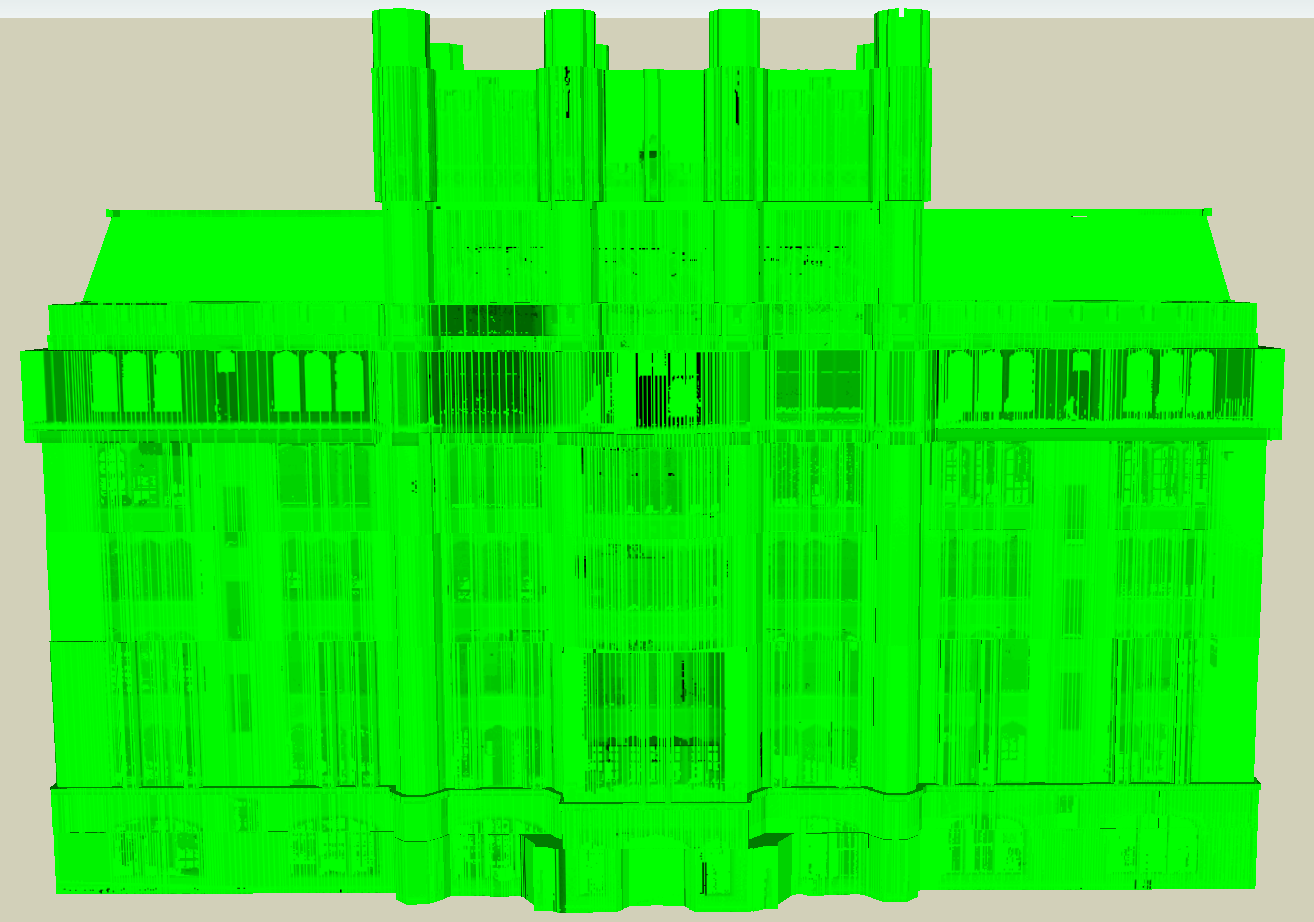
\includegraphics
        [width=0.5\textwidth]
	{figures/IR_skp_error_face_1000_32_4_paper.png}
  }
  \centering
  \subfloat[]{
    \label{fig_EM:b} %% label for first subfigure
    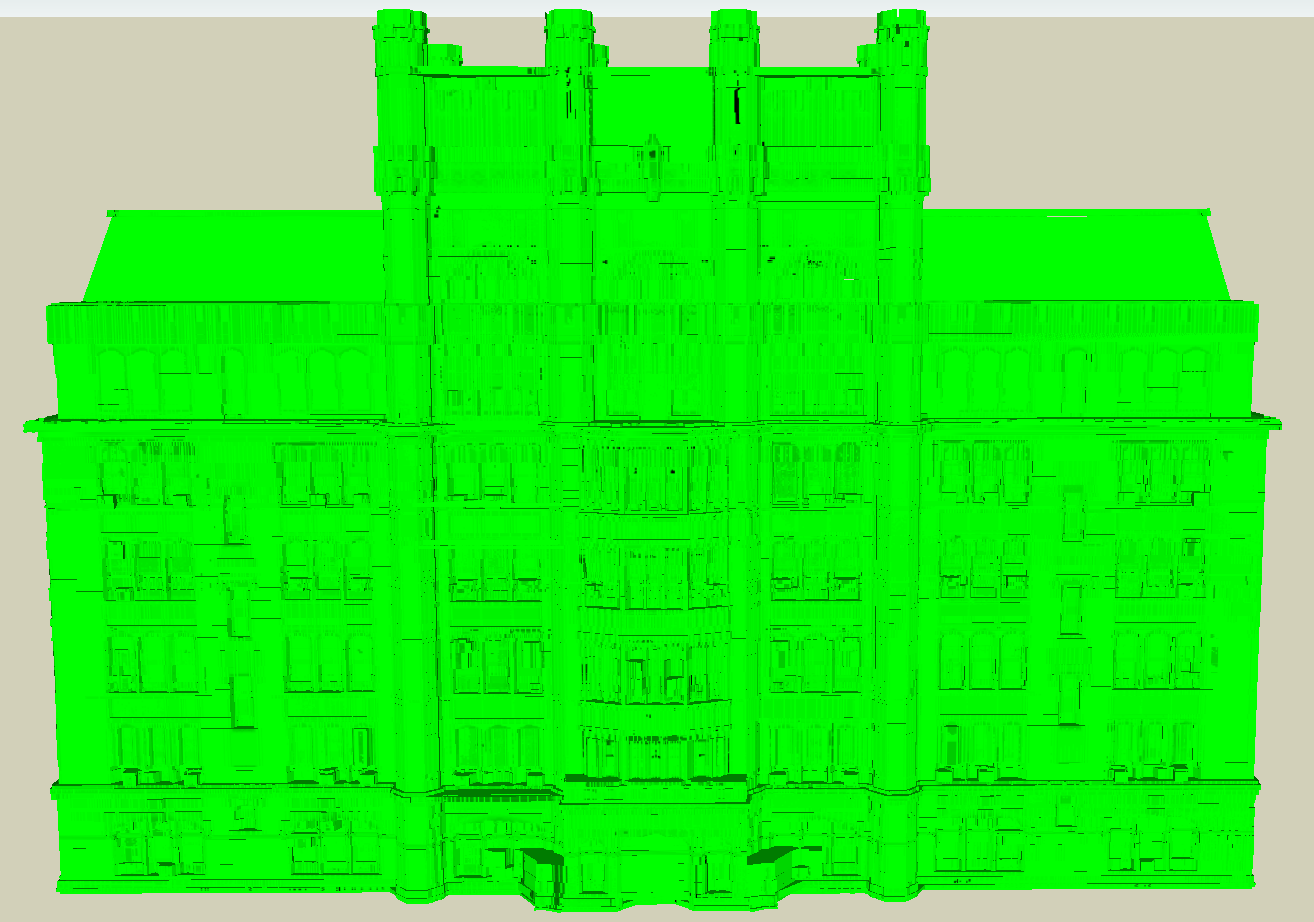
\includegraphics
        [width=0.5\textwidth]
	{figures/IR_skp_error_face_1000_4_1_paper.png}
  }
  \caption{  The deviation mapping of the 3D point cloud. (a) the model built with parameter of
$\tau_r$ = 4 and $\tau_d$ = 32. (b) the model built with parameter of $\tau_r$ = 1 and $\tau_d$ = 4. }
  \label{fig_EM}
\end{figure}
%%% End of Figure


%%%%%%%%%%%%%%%%%%%%%%%%%%%%%%%%
%%%%%%   Discussion %%%%%%%%%%%%
%%%%%%%%%%%%%%%%%%%%%%%%%%%%%%%%
%\section{Discussion}
\label{sec_discussion}


%%%%%%%%%%%%%%%%%%%%%%%%%%%%%%%%
%%%%%%   All Figures     %%%%%%%
%%%%%%%%%%%%%%%%%%%%%%%%%%%%%%%%
%%% Refer to epslatex.pdf:pp106

\ifthenelse{\equal{\twocol}{true}}{
%\newpage % TWO COLUMN VERSION
}{
\newpage % TWO COLUMN VERSION
}
\section{Practical Aspects and Timeline}

In the processing of implementing the algorithm to obtain the preliminary results, we gained in-depth
knowledge of the 3D tools and related programming language. The whole project consists of over 20000
lines of C++ code and over 1000 lines of Ruby code of Google SketchUp plug-ins for model visualization.
Based on the work has been done and this code base, we believe that the remaining research will
progress fast and the dissertation defense will be in July 2009.

The remaining research problems include the following:
\begin{enumerate}
\item Apply the approach on synthetic data. This will help us to have a better view on the final model. We have
already developed another tool which takes a 3D model and produces synthetic 3D point cloud. This tool provides
us a ground truth for the comparison.
\item Apply the approach on more real data. This includes not only exterior scanning of a building but also
interior scanning of it.
\end{enumerate}

All the above work will ensure that our proposed technique is useful for web-based 3D modeling applications.

%%%THESIS - Discussion
%We presented a light-weight based 3D building model reconstruction from range data obtained
%by laser scanner. Our work is based on the observation that each man-made building can be
%viewed as the combination of two basic components, the extruded and the tapered components.
%Based on the above observation, to reconstruct 3D structure of a building from its point cloud,
%we need only to identify the extruded and tapered components and represent them in a way
%similar to procedural modeling language for quickly reconstruction or navigation.
%
%The inference process is based on 2D sliced images obtained by projecting 3D point cloud data.
%
%
%The benefits of converting 3D point cloud to 3D model representation include:
%1. The storage space is much more efficient. To store point cloud data of a building,
%it takes 700+ MB in text format. Even though we can convert this
%to binary and compress it to ZIP format, it still takes more than 200 MB to store the data.
%This makes the web-based application almost impossible. After applying our algorithm
%on this, the IR ASCII file only takes less than 100 KB to represent the same building.
%2. The geometry of the building is inferred and therefore it can directly treated as
%3D model and easily be displayed in any 3D visualization tools, such as Google Earth. This
%is illustrated in Figure \ref{fig_IR_2_DXF}.
%
%The remaining work is to apply the approach to more real data, including interior scanning
%of a building.
%
%Also to do a controlled experiment, we are planning to applying the approach to synthetic
%data. We have an existed tool to generate 3D range data from model, which provide us a golden
%truth for comparison.

%%%%%%%%%%%%%%%%%%%%%%%%%%%%%%%%
%%%%%%   Bibliography %%%%%%%%%%
%%%%%%%%%%%%%%%%%%%%%%%%%%%%%%%%
\newpage
\bibliography{report}
\bibliographystyle{unsrt}
%\bibliographystyle{alpha}
%\bibliographystyle{plain}

%\begin{thebibliography}{199}
%
%\bibitem{Sym_PSGRF}
%  \bbauth{J. Podolak, P. Shilane, A. Golovinskiy, S. Rusinkiewicz and T. Funkhouser},
%  \bbtitl{A Planar-Reflective Symmetry Transform for 3D Shapes},
%  \bbjour{Proceedings of ACM SIGGRAPH},
%  pp. 549 - 559, 2006
%
%\bibitem{Sym_ZPA}
%  \bbauth{H. Zabrodsky, S. Peleg, and D. Avnir},
%  \bbtitl{Symmetry as a Continuous Feature},
%  \bbjour{IEEE Pattern Analysis and Machine Intelligence},
%  Vol 17, No. 12, December 1995
%
%\bibitem{Sym_TW}
%  \bbauth{S. Thrun and B. Wegbreit},
%  \bbtitl{Shape from Symmetry},
%  \bbjour{Proceedings of the Tenth IEEE International Conference on Computer Vision (ICCV) },
%  2005
%
%\bibitem{Sym_MGP}
%  \bbauth{N. Mitra, L. Guibas and M. Pauly},
%  \bbtitl{Partial and Approximate Symmetry Detection for 3D Geometry},
%  \bbjour{Proceedings of ACM SIGGRAPH}
%  Vol. 25, pp. 560 - 568, 2006
%
%\bibitem{IR_Brown}
%  \bbauth{L.G. Brown},
%  \bbtitl{A survey of image registration techniques},
%  \bbjour{ACM Computing Surveys},
%  Vol. 24, pp. 326 - 376, 1992
%
%\bibitem{IR_ZF}
%  \bbauth{B. Zitova and J. Flusser},
%  \bbtitl{Image Registration Methods: A Survey},
%  \bbjour{Image and Vision Computing},
%  21, pp. 977 - 1000, 2003
%
%\bibitem{IR_HKR}
%  \bbauth{D.P. Huttenlocher, G.A. Klanderman and W.J. Rucklidge},
%  \bbtitl{Comparing images using the Hausdorff distance},
%  \bbjour{IEEE Transactions on Pattern Analysis and Machine Intellinence},
%  Vol. 15, pp. 850 - 863, 1993
%
%\bibitem{PMB_MWH}
%  \bbauth{Pascal Mueller, Peter Wonka, Simon Haegler, Andreas Ulmer and Luc Van Gool},
%  \bbtitl{Procedural Modeling Of Buildings},
%  \bbjour{ACM Transactions on Graphics (TOG)},
%  pp. 614 - 623, 2006
%
%\bibitem{PMB_WWS}
%  \bbauth{Peter Wonka, Michael Wimmer, Fran�ois Sillion and William Ribarsky},
%  \bbtitl{Instant Architecture},
%  \bbjour{ACM SIGGRAPH},
%  pp. 669 - 677, 2003
%
%\bibitem{PMB_PM}
%  \bbauth{Yoav I. H. Parish and Pascal M\"{u}ller},
%  \bbtitl{Procedural modeling of cities},
%  \bbjour{ACM SIGGRAPH},
%  pp. 301 - 308, 2001
%
%\bibitem{RDP_LS}
%  \bbauth{L. Liu and I. Stamos},
%  \bbtitl{Automatic 3D to 2D Registration for The Photorealistic Rendering of Urban Scenes},
%  \bbjour{IEEE Computer Vision and Pattern Recognition},
%  Vol. 2, pp. 137 - 143, June 2005
%
%\bibitem{RDP_LSYGS}
%  \bbauth{L. Liu, I. Stamos, G. Yu, G, Wolberg and S. Zokai},
%  \bbtitl{Multiview Geometry for Texture Mapping 2D Images Onto 3D Range Data},
%  \bbjour{IEEE Computer Vision and Pattern Recognition},
%  Vol. 2, pp. 2293 - 2300, July 2006
%
%\bibitem{RDP_LRS}
%  \bbauth{Leica Geosystems},
%  \bbtitl{http://hds.leica-geosystems.com/}.
%
%\bibitem{CTE_GML}
%  \bbauth{GML Homepage},
%  \bbtitl{http://www.generative-modeling.org/}.
%
%\bibitem{BPA_BMRS}
%  \bbauth{F. Bernardini, J. Mittlelman, H. Rushmeir and C. Silva},
%  \bbtitl{The ball-pivoting algorithm for surface reconstruction},
%  \bbjour{IEEE Transaction on Visualization and Computer Graphics},
%  Vol. 5, n. 8, pp. 349 - 359, 1999
%
%\bibitem{BPA_MVL}
%  \bbauth{E. Medeiros, L. Velho and W. Lopes},
%  \bbtitl{Restricted BPA: applying ball-pivoting on the plane},
%  \bbjour{IEEE Proceedings on Computer Graphics and Image Processing},
%  pp. 372 - 379, Octobor, 2004
%
%\bibitem{DP_DP}
%  \bbauth{D. Douglas and T. Peucker},
%  \bbtitl{Algorithms for the reduction of the number of points required for represent a digitzed line or its caricature},
%  \bbjour{Canadian Cartographer},
%  Vol. 10(2), pp. 112 - 122, 1973
%
%\bibitem{DP_WM}
%  \bbauth{S. Wu and M. R. G. Marquez}
%  \bbtitl{A non-self-intersection Douglas-Peucker algorithm},
%  \bbjour{IEEE Proceedings on Computer Graphics and Image Processing},
%  pp. 60 - 66, 2003
%
%\bibitem{DP_HS}
%  \bbauth{J. Hershberge and  J. Snoeyink},
%  \bbtitl{Speeding Up the Douglas-Peucker Line-Simplification Algorithm},
%  \bbjour{Proceedings of 5th International Symposium Spatial Data Handling},
%  pp. 134 - 143, 1992
%
%\bibitem{DP_OWYC}
%  \bbauth{S. Or, K. Wong, Y. Yu and M. Chang},
%  \bbtitl{Highly Automatic Approach to Architectural Floorplan Image Understanding and Model Generation},
%  \bbjour{Proceedings of Vison, Modeling, and Visualization}
%  Nov. 2005
%
%\bibitem{DP_AAKMT}
%  \bbauth{B. Aronov, T. Asano, N. Katoh, K. Mehlhorn, and T. Tokuyama},
%  \bbtitl{Polyline Fitting of Planar Points under Min-Sum Criteria},
%  \bbjour{International Journal of Computational Geometry and Applications},
%  Vol. 16, pp. 97 - 116, 2006
%
%\bibitem{RE_TOGSH}
%  \bbauth{W. Thompson, J. Owen, H. J. Germain, S. R. Stark and T. C. Henderson},
%  \bbtitl{Feature-Based Reverse Engineering of Mechanical Parts},
%  \bbjour{IEEE Transactions on Robotics and Automation},
%  Vol. 15, No. 1, February 1999
%
%\bibitem{RE_Fisher}
%  \bbauth{Robert B. Fisher},
%  \bbtitl{Applying knowledge to reverse engineering problems},
%  \bbjour{Computer-Aided Design},
%  Vol. 36, pp. 501 - 510, 2004
%
%\bibitem{RE_CLF}
%  \bbauth{U. Castellani, S. Livatino and R. B. Fisher},
%  \bbtitl{Improving Environment Modeling by Edge Occlusion Surface Completion},
%  \bbjour{Proc. Int. Symp. on 3D Data Processing Visualization and Transmission (3DPVT)},
%  pp. 672 - 675, 2002
%
%\bibitem{RE_WWLZ}
%  \bbauth{Y. F. Wu, Y. S. Wong, H. T. Loh and Y. F. Zhang},
%  \bbtitl{Modeling cloud data using an adaptive slicing approach},
%  \bbjour{Computer-Aided Design}
%  Vol. 36, pp. 231 - 240, 2004
%
%\bibitem{RE_CD}
%  \bbauth{L. D. Cohen and T. Deschamps},
%  \bbtitl{Multiple contour finding and perceptual grouping using minimal paths},
%  \bbjour{Journal of Mathematical Imaging and Vision},
%  Vol. 14, pp. 225 - 236, 2001
%
%\bibitem{RDP_RTW}
%  \bbauth{R. T. Whitaker},
%  \bbtitl{A level-set approach to 3d reconstruction from range data},
%  \bbjour{International Journal of Computer Vision},
%  Vol. 29, pp. 203 - 231, 1998
%
%\bibitem{MIR_FJS}
%  \bbauth{F. J. Sigworth},
%  \bbtitl{A Maximum-Likelihood Approach to Single-Particle Image Refinement},
%  \bbjour{Journal of Structual Biology},
%  pp. 328 - 339, 1998
%
%\bibitem{MIR_BMMNB}
%  \bbauth{I. Braude, J. Marker, K. Museth, J. Nissanov and D. Breen},
%  \bbtitl{Contour-Based Surface Reconstruction using Implicit Curve Fitting, and Distance Field Filtering and Interpolation},
%  \bbjour{In Proc. International Workshop on Volume Graphic},
%  pp. 95 - 102, 2006
%
%\bibitem{MIR_KL}
%  \bbauth{A. B. Konovalov and V. V. Lyubimov},
%  \bbtitl{High-resolution restoration of diffuse optical images reconstructed by the photon average trajectories method},
%  \bbjour{Society of Photo-Optical Instrumentation Engineers (SPIE) Conference Series},
%  Vol. 5474, pp. 66 - 79, 2004
%
%\bibitem{MIR_SKJ}
%  \bbauth{Alexei A. Samsonov, Eugene G. Kholmovskib and Chris R. Johnson},
%  \bbtitl{Image Reconstruction from Sensitivity Encoded MRI Data Using Extrapolated Iterations of Parallel Projections onto Convex Sets},
%  \bbjour{Medical Imaging},
%  Vol. 5032, pp. 1829 - 1838, 2003
%
%\bibitem{MIR_SMHC}
%  \bbauth{C.O.S. Sorzano, R. Marabini, G.T. Herman and J.M. Carazo},
%  \bbtitl{Multiobjective algorithm parameter optimization using multivariate statistics},
%  \bbjour{Pattern recognition},
%  Vol. 38, pp. 2587 - 2601, 2005
%
%\bibitem{MIR_BVC}
%  \bbauth{R. Barbuzza, M. V\'{e}nere and A. Clausse},
%  \bbtitl{Tomographic reconstruction using heuristic Monte Carlo methods},
%  \bbjour{Journal of Heuristics},
%  Vol. 13, Issue 3, pp. 227 - 242, June 2007

%\bibitem{DIP_Pratt}
%  \bbauth{W.K. Pratt},
%  \bbtitl{Digital Image Processing},
%  \bbjour{Second Ed., Wiley, New York},
%  1991

%\bibitem{
%  \bbauth{
%  \bbtitl{
%  \bbjour{


%\end{thebibliography}

\newpage

%%%%%%%%%%%%%%%%%%%%%%%%%%%%%%%%
%%%%%%   COMMENTS %%%%%%%%%%%%%%
%%%%%%%%%%%%%%%%%%%%%%%%%%%%%%%%
%\section*{Comments}
%\begin{enumerate}
%\item Think about a global scale factor $S$ for zooming, which should be applied to
%  all equations in the rest of the processing.
%\item All the comments for Thesis is put into \%\%\%THESIS\%\%\%
%\item Move the final results to the beginning for attraction.
%\item Cross-correlation explanation.
%\item Insert algorithm table for adaptive BPA, with refinement version of BPA
%\end{enumerate}


%%%%%%%%%%%%%%%%%%%%%%%%%%%%%%%%
%%%%%%   Figures $%%%%%%%%%%%%%%
%%%%%%%%%%%%%%%%%%%%%%%%%%%%%%%%

%%%%%%%%%%%%%%%%%%%%%%%%%%%%%%%%
\end{document}
